\documentclass[12pt]{article}
\usepackage[utf8]{inputenc}
\usepackage[T1]{fontenc}
\usepackage{lmodern}
\usepackage[left=1in,right=1in,top=1.5in,bottom=1.5in]{geometry}
\usepackage{setspace}
\onehalfspacing
\usepackage{amsmath,amssymb,amsthm,mathtools,bm}
\usepackage{booktabs,tabularx,longtable,array,multirow}
\usepackage{enumitem}
\setlist{noitemsep,topsep=3pt,parsep=0pt,partopsep=0pt}
\usepackage{graphicx}
\usepackage{xcolor}
\usepackage[round]{natbib}
\usepackage{hyperref}
\usepackage[nameinlink,noabbrev]{cleveref}
\usepackage{fancyhdr}
\usepackage{tikz}
\usetikzlibrary{arrows.meta,positioning,shapes.geometric}

\hypersetup{
    colorlinks=true,
    linkcolor=blue!70!black,
    citecolor=blue!70!black,
    urlcolor=blue!70!black,
    pdftitle={From Human Markets to Machine Markets: Feedback Stability, Auditable Memory, and Financial Constraints},
    pdfauthor={Pratik Niroula and Prashant Niroula}
}

\newtheorem{theorem}{Theorem}[section]
\newtheorem{proposition}[theorem]{Proposition}
\newtheorem{lemma}[theorem]{Lemma}
\newtheorem{corollary}[theorem]{Corollary}
\theoremstyle{definition}
\newtheorem{definition}[theorem]{Definition}
\theoremstyle{remark}
\newtheorem{remark}[theorem]{Remark}

\newcommand{\R}{\mathbb{R}}
\newcommand{\E}{\mathbb{E}}
\newcommand{\norm}[1]{\left\lVert #1\right\rVert}
\newcommand{\diag}{\operatorname{diag}}
\newcommand{\tr}{\operatorname{tr}}
\newcommand{\Cov}{\operatorname{Cov}}
\newcommand{\Var}{\operatorname{Var}}

\renewcommand{\topfraction}{0.90}
\renewcommand{\bottomfraction}{0.80}
\renewcommand{\textfraction}{0.10}
\renewcommand{\floatpagefraction}{0.85}

% Import generated macros
% Historical macro import retired after current-source reconstruction.
% Historical macro import retired after current-source reconstruction.
% Historical macro import retired after current-source reconstruction.

\pagestyle{fancy}
\fancyhf{}
\fancyhead[L]{\footnotesize Niroula and Niroula}
\fancyhead[R]{\footnotesize From Human Markets to Machine Markets}
\fancyfoot[C]{\thepage}
\setlength{\headheight}{15pt}

\title{\textbf{From Human Markets to Machine Markets:}\\[0.3em]
\Large Feedback Stability, Auditable Memory, and Financial Constraints}
\author{\textbf{Pratik Niroula}\thanks{Current affiliation pending author confirmation. Email: \texttt{pratik.niroula@alumni.harvard.edu}.} \quad and \quad \textbf{Prashant Niroula}\thanks{Current affiliation pending author confirmation. Email: \texttt{prashant.niroula@alumni.harvard.edu}.}}
\date{\today}

\begin{document}

\maketitle
\thispagestyle{empty}

\vspace{-0.5em}
\begin{abstract}\noindent We study identification of adaptive memory under financially constrained probing. For a known symmetric cohort pair, deterministic reset probes without process noise require executed quantity of order $\delta^{-2}$ and solvent trader capital of order $\delta^{-4}$ under noisy-price observations. We prove attainable bounds and show how financial disclosure or natural excitation changes the experiment. Reconstruction of 768 market study units reveals timing and filter sensitivity and rejects maintained covariance restrictions. Financial replays distinguish inventory limits from defaults. These results define conditional information contracts rather than identify participant-level learning or certify operational market safety.\end{abstract}

\vspace{1.0em}
\noindent\textbf{Keywords:} Adaptive learning, algorithmic trading, financial stability, market microstructure, system identification, non-normal dynamics, Kreiss constant.\\
\textbf{JEL Classification Codes:} G01, G10, G14, C32, C58, D83.

\clearpage
\thispagestyle{empty}
\section*{Disclosure Statement: Pratik Niroula}
\noindent\textbf{Author-provided declaration; review draft.} This format candidate is not ready for submission. Current affiliations/status remain unknown. The authors declare equal contribution, no external research funding and no conflicts; scientific review and final submission checks remain open.

\noindent Pratik Niroula and Prashant Niroula contributed equally. No external research funding was received. No conflicts of interest are declared.

\clearpage
\thispagestyle{empty}
\section*{Disclosure Statement: Prashant Niroula}
\noindent\textbf{Author-provided declaration; review draft.} Pratik Niroula and Prashant Niroula contributed equally. No external research funding was received. No conflicts of interest are declared.

\noindent A separate AI-assistance and source/rights record accompanies this review candidate. Author responsibility and journal submission declarations require confirmation before submission.

\clearpage
\setcounter{page}{1}

\section{Introduction}
\label{sec:intro}

Electronic execution and market making raise a financial identification question: what can aggregate price and flow observations reveal about trading rules, and which financial constraints govern experiments intended to learn those rules? Microstructure research documents the interaction of trades, quotes and automated liquidity provision \citep{hasbrouck1991,menkveld2013,budish2015}. We study a declared linear feedback economy and its information/resource contracts, then test whether observable measurement diagnostics support the corresponding interpretation.

When trading algorithms condition their order submission and quote-placement decisions on recent transaction prices, prevailing order book imbalances, and trade innovations, the price-formation process ceases to be an open-loop mechanism driven purely by exogenous informational updates regarding fundamentals. Instead, price formation becomes an autonomous \emph{closed-loop dynamical system}: trading decisions generate endogenous price impact, and the resulting price adjustments directly feed back into the learning rules, momentum filters, risk-budgeting heuristics, and execution programs of competing market participants \citep{bouchaud2004fluctuations,cont2010stochastic,cont2014}. 

This closed-loop structural reality was dramatically underscored by major episodic disruptions in electronic markets over the past decade and a half. While disruptions such as the May 6, 2010 Flash Crash in the E-mini S\&P 500 and the October 15, 2014 Treasury flash rally provide compelling historical motivation for analyzing how algorithmic feedback can rapidly deplete liquidity, direct empirical investigation of these episodes is constrained by the non-public nature of regulatory account registries. Modern electronic cryptocurrency order books provide an ideal, transparent empirical testing ground. Electronic cryptocurrency venues provide public trade and book data, but these records do not identify the fraction of activity generated by adaptive algorithms. The supplied samples have the clocks and coverage described below; they do not establish universal nanosecond observation or the absence of off-exchange execution. We therefore exploit high-frequency cryptocurrency order books (complemented by a supplied equity representation whose normalized-source transformation now reproduces exactly, while company-label mapping and physical scale remain unresolved) as an empirical testing ground for our broader theoretical framework.

These information and financial questions concern financial economists, central banks, and market regulators with an urgent, foundational question:
\begin{quote}
\centering
\emph{Can observable market data identify destabilizing adaptive feedback, when does that feedback become financially dangerous, and what information is fundamentally missing from public surveillance data?}
\end{quote}

In this paper, we address this question directly by integrating realization-theoretic system identification with empirical limit order book econometrics and balance-sheet financial constraints. Rather than making speculative assertions regarding black-box artificial intelligence, we organize our theoretical and empirical findings around \textbf{two foundational pillars}:

\paragraph{Pillar 1: Observable Feedback Does Not Imply Identifiable Machine Behavior.}
We identify the merged rate--weight representation under the modeled reset price-response contract, with known anchor and impact (Theorem~\ref{thm:m1_equivalence}). The resource comparison establishes necessary and sufficient quantity order $\delta^{-2}$ for a known symmetric pair and horizon order $\delta^{-4}$ under average power (Theorem~\ref{thm:resource_frontier}). Actual trading cost gives matching capital order $\delta^{-4}$ for deterministic probes financed by a trader who remains solvent after temporary impact dissipates, when the statistical observer receives only noisy price states (Theorem~\ref{thm:trader_capital_frontier}). A separate counterparty account gives a sharp robust quantity/margin allowance (Theorem~\ref{thm:cash_capital_frontier}). Waiting cannot compensate for a fixed lifetime executed-quantity budget. The dealer's inventory change creates a quadratic adverse mark, rather than only a fixed linear price exposure. These are distinct input, cash and observation contracts. This is the proposed central advance; general unknown-mixture recovery and adaptive probing remain outside the theorem.

The empirical reconstruction tests observable measurement and model restrictions rather than claiming latent learning identification. In the original 768-unit panel, mean legacy forward-flow $Q=0.0081536$ becomes $0.0003807$ with observed flow; pooled raw-return $Q=-0.0001625$ has a date interval including zero. The recorder timing comparison is a different sample and is reported separately. Maintained covariance restrictions reject, and the fee-schedule exercise is a one-treated-asset descriptive association with covariance-sensitive uncertainty. These findings establish why a public reduced-form coefficient cannot be substituted for the controlled information contract.

\paragraph{Pillar 2: Dynamic Eigenvalue Stability Does Not Imply Financial Safety.}
For a fixed initial-disturbance and model-output contract, spectral stability ($\rho(J)<1$) alone does not bound the permitted loss-budget radius. A dealer solvency interpretation additionally requires a justified monetary accounting map. Because the closed-loop market Jacobian $J$ is generically non-normal under asymmetric price-impact and memory parameters (with $J J^\top - J^\top J \neq 0$ except on a measure-zero algebraic subvariety), stable eigenvalues can coexist with large declared-output gain under an appropriate disturbance/output contract. The exact initial-state radius for that declared loss-budget experiment is governed by peak output magnification:
\begin{equation}
r^*_{\text{exact}} = \frac{B}{\sup_{t \ge 0} \|C J^t\|_2} \equiv \frac{B}{M_C},
\end{equation}
which the Kreiss constant $\mathcal{K}(J)$ bounds and the spectral radius completely fails to control (Theorem~\ref{thm:m5_kreiss_solvency}). By Spijker's theorem, under full-state observation ($C = I$), we establish the bilateral bounds:
\begin{equation}
\frac{B}{e \cdot n \cdot \mathcal{K}(J)} \le r^*_{\text{exact}} \le \frac{B}{\mathcal{K}(J)},
\end{equation}
proving that $\frac{B}{e n \mathcal{K}(J)}$ provides a guaranteed safe lower bound, whereas $\frac{B}{\mathcal{K}(J)}$ is an upper bound that must never be mistaken for a conservative safety threshold. The separate lagged-memory experiment reproduces 19,200 paths across 48 cells, but its halt event combines equity and position-limit causes. The 22,000-path funded grid instead has positive-equity inventory-limit events in effective supercritical dynamics. Neither supplies observed market defaults or an independently calibrated policy benefit. Long-run variance and marginal variance are distinct quantities.

\subsection{Related Literature}
Our work bridges four major strands of literature across financial economics, market microstructure, systemic risk, and dynamical systems theory.

\paragraph{High-Frequency Trading and Market Microstructure.}
Beginning with the seminal contributions of \citet{kyle1985continuous} and \citet{glosten1985bid}, classical microstructure models analyze the informational content of order flow and dealer inventory management under asymmetric information. \citet{hasbrouck1991} pioneered the empirical vector autoregressive decomposition of trades and quotes, establishing that trade innovations exert persistent impacts on security prices. \citet{campbell1993trading} demonstrated that trading volume and return serial correlations reflect interactions between liquidity traders and risk-averse market makers.

In modern electronic markets, high-frequency trading firms and automated algorithms dominate liquidity provision and execution \citep{menkveld2013,budish2015,biais2015}. While \citet{hendershott2011does} document that algorithmic trading improves liquidity and narrows bid-ask spreads during normal trading periods, \citet{budish2015} show that continuous double auctions generate socially wasteful latency arms races, and \citet{biais2015} demonstrate that algorithmic speed advantages can lead to adverse selection spirals. We advance this literature by formalizing the closed loop between algorithmic learning rules and endogenous price impact, establishing conditional realization and resource bounds for the declared controlled experiment. Public ticker data require a separate observation and identification argument.

\paragraph{Price Impact and Limit Order Book Dynamics.}
An extensive literature studies price impact, signed-flow memory and quote imbalance \citep{bouchaud2004fluctuations,cont2014}. Our long-run regression diagnostics retain these as competing explanations. Lag controls and observable kernel signs do not identify parent orders, learner policies or contemporaneous structural shocks.

\paragraph{Intermediary Solvency, Funding Liquidity, and Systemic Risk.}
The distinction between market liquidity and funding liquidity is central to modern theories of financial fragility \citep{brunnermeier2009,adrian2010liquidity,he2013intermediary}. When leveraged market makers suffer balance-sheet drawdowns, risk-management constraints (such as Value-at-Risk limits or regulatory margin requirements) force them to withdraw quotes, widening spreads and amplifying price dislocations \citep{greenwood2015vulnerable,eisenberg2001systemic}. Our conditional loss-output analysis separates spectral stability from a declared loss budget. The empirical studies do not demonstrate intermediary insolvency in a calibrated stable market; the positive price-only response has the more restrictive geometry proved below.

\paragraph{Non-Normal Dynamics and the Kreiss Matrix Theorem.}
Non-normal transients and Kreiss bounds are established mathematical tools \citep{kreiss1962,spijker1991,trefethen2005spectra}. Their application to financial bubbles also precedes this paper: \citet{sornette2023nonnormal} links subcritical financial dynamics to non-normal networks and the Kreiss constant. We therefore do not claim first application to finance. Our proposed contribution connects a particular memory-resolution experiment to executed-quantity and monetary-output resources; the underlying norm and testing tools remain established.

\paragraph{Identification and Experiment Design.}
Known finite hypothesis classes already admit sample-complexity bounds and excitation design \citep{chatzikiriakos2024finite,chatzikiriakos2026active}. The latter studies fully observed states with Gaussian process noise and bounded average input power. Our price-observation experiment instead specifies lifetime executed quantity, eventual-solvency capital and richer financial-disclosure boundaries in a noiseless-state cohort model. These are contract and resource distinctions to assess against established identification theory; we do not claim first finite-model testing or constrained excitation.

\begin{table}[htbp]
\centering\footnotesize
\caption{Comparison of Microstructural Frameworks and Surveillance Assumptions.}
\label{tab:lit_comparison}
\begin{tabularx}{\textwidth}{p{3.2cm}Xp{2.2cm}XX}\toprule
Model / Paradigm & Information Architecture & Dynamics & Stability Metric & Surveillance Scope \\\midrule
\citet{kyle1985continuous} & Informed vs.\ noise flow & Single-auction & Linear pricing $\lambda$ & Adverse selection \\
\citet{hasbrouck1991} & Trades and quotes (VAR) & Joint response & Cumulative IRF & Permanent price impact \\
\citet{bouchaud2004fluctuations} & Signed order flow memory & Propagator & Kernel decay & Meta-order splitting \\
\citet{cont2014} & Multi-level order book & Static regression & $R^2$ of OFI & Short-term price discovery \\
\citet{brunnermeier2009} & Leveraged margin financing & Nonlinear spiral & Margin constraints & Liquidity spirals \\
\textbf{This Paper} & Defined reset probe & Merged memory & Quantity/output budget & Known-pair resource orders \\\bottomrule
\end{tabularx}
\end{table}

Financial exploration already balances trading cost and information. \citet{parkvanroy2012} study learning impact coefficients during execution, with known distinct transient decay rates and an adaptive expected-regret objective. Here the known-pair diagnostic concerns coalescing latent adaptation rates and an explicit initial-capital/solvency restriction under a specified observation law. The paper does not claim a first financial learning algorithm or a new general exploration-cost principle. Positive transaction-cost and no-dynamic-arbitrage conditions likewise precede this work \citep{gatheral2010,schneiderlillo2017}; the contribution must lie in the particular model/resource connection and its demonstrated scope.

Price-trajectory information and impact estimation also have prior work. \citet{li2024trajectory} compare regular-model Fisher information under different price sampling schemes. Our singular known-pair test asks about separation-dependent probing and capital, rather than a generally superior sampling method. The average-book quadratic execution cost and positive-kernel criterion are likewise established \citep{alfonsi2016matrix}; the positive-cohort lemma verifies that this particular response fits that geometry, rather than proposing a new no-manipulation criterion.

\subsection{Empirical Research Design and Setting}
We retain the original multi-year panel, recorder timing/filter comparison, joint cross-venue VAR, liquidity-state regressions, supplied equity representation, financial simulations and forecast diagnostics. Each has its own clock, sample and inference assumptions. Existing raw files and outputs are reconstructed before interpreting mechanisms. The paper distinguishes an observed coefficient, a maintained-model test, a constructed financial scenario and a controlled identification theorem. Data/provider and calibration boundaries accompany the results; they are not inferred from a successful numerical reproduction.

Theoretical identification and resource bounds appear first, followed by measurement construction and reconstructed empirical studies. The final section gives the finite-window input/output gate and its operational limitations.


\section{Theoretical Model and Identification Boundaries}
\label{sec:model}

\subsection{Microfoundations of Closed-Loop Price Formation}
We formalize an electronic financial market sampled at discrete uniform time intervals $t \in \{0, 1, 2, \dots\}$, where time step $\Delta$ represents the operational sampling frequency (e.g., 1 second). Let $p_t$ denote the price level in monetary units of a traded asset, and let $p_t^*$ denote the unobserved fundamental value, which evolves as a martingale:
\begin{equation}
p_{t+1}^* = p_t^* + \xi_{t+1}, \qquad \xi_{t+1} \sim \text{i.i.d.}(0, \sigma_\xi^2).
\label{eq:fundamental_process}
\end{equation}
We define the pricing error (displacement from fundamental) as $x_t \equiv p_t - p_t^*$.

\paragraph{Dealer Pricing, Posted Depth, and Equilibrium Price Impact.}
Following the continuous auction framework of \citet{kyle1985continuous} adapted to discrete order books \citep{glosten1985bid,hasbrouck1991,bouchaud2004fluctuations}, competitive dealers absorb net incoming order flow by posting aggregate limit order depth $D_t > 0$. Total incoming flow combines algorithmic demand $u_t$ and exogenous liquidity noise $\varepsilon_{t+1} \sim \text{i.i.d.}(0, \sigma_\varepsilon^2)$, counterbalanced by fundamentalist arbitrageurs submitting demand $-\varphi x_t$.

The clearing price adjustment across posted depth satisfies:
\begin{equation}
p_{t+1} - p_t = \frac{1}{D_t} \left( u_t - \varphi x_t + \varepsilon_{t+1} \right) \equiv \kappa_t \left( u_t - \varphi x_t + \varepsilon_{t+1} \right),
\end{equation}
where equilibrium price impact $\kappa_t \equiv 1/D_t$ is the structural inverse of available limit depth. Subtracting fundamental increment $\xi_{t+1}$ from both sides yields the pricing error recursion:
\begin{equation}
x_{t+1} = (1 - \kappa_t \varphi) x_t + \kappa_t u_t + \left( \kappa_t \varepsilon_{t+1} - \xi_{t+1} \right).
\end{equation}
Defining direct price persistence $a_t \equiv 1 - \kappa_t \varphi \in [0, 1)$ and combined innovation $w_{t+1} \equiv \kappa_t \varepsilon_{t+1} - \xi_{t+1}$, we obtain the foundational pricing equation (evaluated at steady-state depth $D^*$, with $\kappa \equiv 1/D^*$):
\begin{equation}
x_{t+1} = a x_t + \kappa u_t + w_{t+1}, \qquad w_{t+1} \sim \text{i.i.d.}(0, \sigma_w^2).
\label{eq:micro_pricing}
\end{equation}
When fundamentalist arbitrage is strong ($\varphi \to 1/\kappa$), $a \to 0$ and prices immediately reflect fundamentals. For fixed $\varphi$, decreasing depth increases $\kappa$ and decreases $a=1-\kappa\varphi$; it does not make $a$ approach unity. Maintaining $0\le a<1$ requires $0<\kappa\varphi\le1$. An endogenous arbitrage response would require its own economic specification.

\paragraph{Algorithmic Learning Microfoundations.}
We consider $K$ heterogeneous cohorts of algorithmic traders. Each cohort $i \in \{1, \dots, K\}$ maintains an internal state variable $y_{i,t} \in \R$ representing its estimate of price momentum, trend, or fundamental mispricing. The specified Kalman and regularized gradient models give exponential-memory recursions. Embedding either in the price-first cohort economy additionally requires the stated signal, gain and timing assumptions; the empirical regressions do not identify that embedding.

\begin{proposition}[Steady-State Kalman Filtering Yields Exponential Memory]
\label{prop:kalman}
As an independent microfoundation for exponential-memory signals, suppose an algorithmic execution desk tracks a latent local trend $v_t \in \R$ following a random walk $v_{t+1} = v_t + \zeta_{t+1}$ with independent centered Gaussian innovations of variance $\sigma_\zeta^2>0$, observing $r_t=v_t+\nu_t$ with independent centered Gaussian observation noise of variance $\sigma_\nu^2>0$. Assume a Gaussian initial state and the steady-state prior covariance. The minimum mean-squared error (MMSE) estimator is given by the steady-state Kalman filter recursion:
\begin{equation}
\hat{v}_{t+1} = (1 - \eta) \hat{v}_t + \eta r_t,
\label{eq:kalman_recursion}
\end{equation}
where the steady-state Kalman gain $\eta \in (0, 1)$ is the unique positive root of the algebraic Riccati equation:
\begin{equation}
\eta = \frac{-\sigma_\zeta^2 + \sqrt{\sigma_\zeta^4 + 4 \sigma_\zeta^2 \sigma_\nu^2}}{2 \sigma_\nu^2}.
\end{equation}
\end{proposition}

\begin{proof}
The scalar state-space model is $v_{t+1} = v_t + \zeta_{t+1}$ and $r_t = v_t + \nu_t$. Let $P_{\infty}$ denote the steady-state prior error variance. The Riccati equation is $P_\infty = P_\infty - \frac{P_\infty^2}{P_\infty + \sigma_\nu^2} + \sigma_\zeta^2$, which simplifies to $P_\infty^2 - \sigma_\zeta^2 P_\infty - \sigma_\zeta^2 \sigma_\nu^2 = 0$. The unique positive root is $P_\infty = \frac{\sigma_\zeta^2 + \sqrt{\sigma_\zeta^4 + 4\sigma_\zeta^2 \sigma_\nu^2}}{2}$. The steady-state Kalman gain is $\eta = \frac{P_\infty}{P_\infty + \sigma_\nu^2} \in (0, 1)$. Substituting into the update $\hat{v}_{t+1} = \hat{v}_t + \eta (r_t - \hat{v}_t)$ yields \eqref{eq:kalman_recursion}.
\end{proof}

\begin{proposition}[Regularized Online Gradient Descent Yields Exponential Memory]
\label{prop:ogd}
Consider an automated trading agent updating policy weights $\theta_t \in \R$ via Online Gradient Descent (OGD) with $L_2$ weight regularization $\gamma \in (0, 1)$ to minimize a quadratic prediction loss $\mathcal{L}(\theta_t; x_t) = \frac{1}{2} (x_t - \theta_t)^\top H (x_t - \theta_t)$:
\begin{equation}
\theta_{t+1} = (1 - \gamma) \theta_t - \alpha \nabla_\theta \mathcal{L}(\theta_t; x_t),
\end{equation}
where $H>0$ is scalar curvature and $\alpha>0$ is the learning step size. If the effective adaptation rate $\eta \equiv \gamma + \alpha H \in (0, 1)$ and we define gain $q \equiv \frac{\alpha H}{\gamma + \alpha H}$, the parameter recursion is mathematically identical to:
\begin{equation}
\theta_{t+1} = (1 - \eta) \theta_t + \eta q x_t.
\end{equation}
\end{proposition}

\begin{proof}
Differentiating the loss, $\nabla_\theta \mathcal{L} = -H(x_t - \theta_t)$. The parameter update becomes:
$\theta_{t+1} = (1 - \gamma)\theta_t + \alpha H (x_t - \theta_t) = (1 - (\gamma + \alpha H))\theta_t + \alpha H x_t$.
Substituting $\eta = \gamma + \alpha H$ and $q = \frac{\alpha H}{\eta}$ yields $\theta_{t+1} = (1 - \eta)\theta_t + \eta q x_t$.
\end{proof}

Propositions~\ref{prop:kalman} and~\ref{prop:ogd} demonstrate that exponential memory decay is not an ad hoc modeling assumption, but rather a common local linear reduction of standard optimal filtering and regularized gradient optimization.

\paragraph{The Joint Closed-Loop Dynamical System.}
Let cohort $i$ submit demand proportional to its state, $u_{i,t} = q_i y_{i,t}$, where $q_i \in \R$ reflects aggressive capital allocation ($q_i > 0$ represents trend-following / momentum; $q_i < 0$ represents mean-reversion). Total algorithmic demand is $u_t = \sum_{i=1}^K q_i y_{i,t}$. Each cohort updates its internal state according to:
\begin{equation}
y_{i, t+1} = (1 - \eta_i) y_{i, t} + \eta_i x_{t+1}, \qquad \eta_i \in (0, 1).
\label{eq:cohort_update}
\end{equation}

Substituting the market price formation equation \eqref{eq:micro_pricing} into the update rule \eqref{eq:cohort_update}, we obtain:
\begin{equation}
y_{i, t+1} = (1 - \eta_i) y_{i, t} + \eta_i \left( a x_t + \kappa \sum_{j=1}^K q_j y_{j, t} + w_{t+1} \right).
\end{equation}
Stacking the pricing error $x_t$ and the $K$ internal cohort states into the state vector $\mathbf{z}_t = (x_t, y_{1,t}, \dots, y_{K,t})^\top \in \R^{K+1}$, the joint economy forms an autonomous discrete-time linear dynamical system:
\begin{equation}
\mathbf{z}_{t+1} = J \mathbf{z}_t + \mathbf{b} w_{t+1},
\label{eq:state_space_system}
\end{equation}
where the closed-loop system Jacobian matrix $J \in \R^{(K+1) \times (K+1)}$ is given by:
\begin{equation}
J = \begin{bmatrix}
a & \kappa q_1 & \kappa q_2 & \cdots & \kappa q_K \\
\eta_1 a & 1 - \eta_1 + \eta_1 \kappa q_1 & \eta_1 \kappa q_2 & \cdots & \eta_1 \kappa q_K \\
\eta_2 a & \eta_2 \kappa q_1 & 1 - \eta_2 + \eta_2 \kappa q_2 & \cdots & \eta_2 \kappa q_K \\
\vdots & \vdots & \vdots & \ddots & \vdots \\
\eta_K a & \eta_K \kappa q_1 & \eta_K \kappa q_2 & \cdots & 1 - \eta_K + \eta_K \kappa q_K
\end{bmatrix},
\label{eq:full_jacobian}
\end{equation}
and $\mathbf{b} = (1, \eta_1, \eta_2, \dots, \eta_K)^\top$.

\paragraph{Single-Cohort Stability Boundary.}
In the single-cohort case ($K=1$), defining total loop feedback gain $Q \equiv \kappa q_1$, the characteristic polynomial of $J$ is:
\begin{equation}
P(\lambda) = \det(\lambda I - J) = \lambda^2 - \left( a + 1 - \eta + \eta Q \right) \lambda + (1 - \eta) a.
\label{eq:char_poly}
\end{equation}
By the Jury stability criterion, all roots of $P(\lambda)$ lie strictly inside the open unit disk $\{|\lambda| < 1\}$ if and only if $|P(0)| < 1$, $P(1) > 0$, and $P(-1) > 0$. Here $|P(0)| = (1 - \eta)a < 1$ holds for all $a \in [0, 1)$ and $\eta \in (0, 1)$. Evaluating at $\lambda = 1$ and $\lambda = -1$:
\begin{equation}
P(1) = (1 - a - Q) \eta, \qquad P(-1) = (2 - \eta)(1 + a) + \eta Q.
\end{equation}
For the positive-feedback economy ($Q \ge 0$), $P(-1) > 0$ is strictly satisfied, so Schur stability is strictly equivalent to:
\begin{equation}
S \equiv a + Q < 1, \qquad \text{or equivalently} \quad \mathcal{L} \equiv \frac{Q}{1 - a} < 1,
\label{eq:stability_cond}
\end{equation}
where $S$ is total closed-loop persistence and $\mathcal{L}$ is the loop ratio. In the general signed-feedback economy ($Q \in \R$), the full Jury stability interval is $-\frac{(2-\eta)(1+a)}{\eta} < Q < 1 - a$, where the lower bound prevents period-doubling oscillatory explosion. For positive feedback with the stated interior learning and anchor conditions, the $S<1$ boundary is also sufficient under the following one-period lag. Signed-feedback stability must instead use that lagged model's full Jury inequalities. If execution features a discrete one-period lag ($x_{t+1} = a x_t + y_t + w_{t+1}, y_{t+1} = (1 - \eta) y_t + \eta Q x_t$), evaluating $P_{\text{lag}}(1) = (1 - a - Q)\eta > 0 \iff S \equiv a + Q < 1$, identically.

\subsection{Identification Boundaries: Merged Rate-Weight Equivalence and Separation Complexity}
A central question in algorithmic market surveillance is whether an econometrician observing public trade executions and prices can identify the individual algorithmic strategies active in the market.

\begin{theorem}[Merged Rate-Weight Equivalence and Minimax Separation Complexity]
\label{thm:m1_equivalence}\label{thm:m2_sample_complexity}
Let price impact $\kappa > 0$ and anchor $a \in [0, 1)$ be known. Use zero initial states and a common specified innovation/probe contract, and observe the modeled price state $x_t$. This contract is distinct from assuming that an anonymous market midpoint reveals fundamental pricing error.
\begin{enumerate}
    \item \textbf{Exact Equivalence Class:} Two market economies $\mathcal{E}_A = \{(q_i^A, \eta_i^A)\}_{i=1}^{K_A}$ and $\mathcal{E}_B = \{(q_i^B, \eta_i^B)\}_{i=1}^{K_B}$ generate mathematically identical modeled price-state responses $x_t$ for all $t \ge 0$ under all public probing sequences $\{u_t^{\text{probe}}\}_{t \ge 0}$ if and only if their merged rate--weight measures coincide:
    \begin{equation}
    \sum_{i: \eta_i^A = \eta} q_i^A = \sum_{j: \eta_j^B = \eta} q_j^B \qquad \forall \eta \in (0, 1).
    \label{eq:merged_measure}
    \end{equation}
    The minimal state-space realization dimension is $1 + |\operatorname{supp}(\mathcal{M})|$, where $|\operatorname{supp}(\mathcal{M})|$ counts distinct rates with nonzero merged weights after signed cancellations, rather than every latent cohort. These are dynamic adaptation rates $\eta_i \in (0, 1)$ (any instantaneous cohort with $\eta = 1$ merges directly into the feedforward anchor $a$ without adding a dynamic pole).
    \item \textbf{Minimax Separation Complexity:} Consider testing whether a noiseless-state market ($w_t = 0$) consists of a single merged cohort with rate $\bar{\eta}$ versus two split cohorts with rates $\bar{\eta} \pm \delta$ and identical nonzero total feedback $Q$, splitting its weight symmetrically. Work on a fixed compact family whose transitions are uniformly Schur stable, with rates bounded away from zero and one and $\sigma_v>0$. Under deterministic probing with $\mathcal P_{\text{probe}}>0$ satisfying the power constraint $\frac{1}{T} \sum_{t=0}^{T-1} u_t^2 \le \mathcal{P}_{\text{probe}}$ and independent additive Gaussian observation noise $\tilde{x}_t = x_t + v_t$ with $v_t \sim \mathcal{N}(0, \sigma_v^2)$, any deterministic/open-loop probing sequence satisfying the stated average-power constraint distinguishing the two economies with worst-case probability of error at most $\alpha \in (0, 1/4)$ requires an observation budget $T$ satisfying:
    \begin{equation}
    T \ge \frac{C(\alpha, \sigma_v, \mathcal{P}_{\text{probe}},\mathcal F)}{\delta^4} = \Omega(\delta^{-4}),
    \label{eq:delta_fourth}
    \end{equation}
    where $C(\alpha, \sigma_v, \mathcal{P}_{\text{probe}},\mathcal F) > 0$ is a constant independent of $\delta$.
\end{enumerate}
\end{theorem}

\begin{proof}
Let $r_i=1-\eta_i$. Zero-state cohort recursion gives
\[G(z)=\sum_i\frac{q_i\eta_i z}{z-r_i},\qquad H(z)=\frac{\kappa}{z-a-\kappa G(z)}.\]
Equality of every controlled price response is equality of $H$, which recovers $G$ because $a,\kappa$ are known. Its residue at a retained rate is $r_i\eta_i$ times that rate's merged weight. Distinct nonzero residues identify the merged measure by uniqueness of partial fractions. Conversely identical merged measures give identical $G,H$ and responses. After signed cancellations, let $D(z)$ be the product of the retained distinct $(z-r_i)$ factors. The numerator of $H$ is $\kappa D$ and its denominator has degree one more. At any retained $r_i$, the denominator is nonzero because its residue, $r_i$ and $\eta_i$ are nonzero. Thus no common factor remains and the minimal realization has the claimed degree. The cohort poles are poles of $G$ and zeros of $H$, not its closed-loop poles.

For the symmetric pair write $q=Q/\kappa$. Direct algebra gives
\[G_\delta-G_0=-\frac{qz(z-1)\delta^2}{(z-1+\bar\eta)((z-1+\bar\eta)^2-\delta^2)}.\]
All three denominator factors on $|z|=1$ have modulus at least the declared rate separation from the endpoints, say $\epsilon$. Compactness and uniform Schur stability give a finite bound $M=\sup_{\theta\in\mathcal F,|z|=1}|H_\theta(z)|$. The identity $H_\delta-H_0=H_\delta H_0(G_\delta-G_0)$ therefore gives induced $\ell_2$ gain at most $K\delta^2$, where $K=2|q|M^2/\epsilon^3$. Zero-padding the finite probe and retaining its observed response cannot increase that gain. Its Gaussian mean difference consequently has squared norm at most $K^2\delta^4\mathcal P_{probe}T$, and equal-noise KL is at most $K^2\delta^4\mathcal P_{probe}T/(2\sigma_v^2)$. Error at most $\alpha$ requires total variation at least $1-2\alpha$. Pinsker then yields
\[T\ge\frac{4\sigma_v^2(1-2\alpha)^2}{K^2\mathcal P_{probe}\delta^4}.\]
The constant depends on the specified family and resources, rather than being universal. The following theorem gives matching known-pair resource orders and explicit financial contracts.
\end{proof}

\begin{remark}[Scope of the Identification Result]
The result concerns the stated model and observation contract. Cohorts sharing an exact rate enter the price response through their merged weight; this does not determine participant identities or wealth allocations. Nearby rates can be distinguishable with sufficient information. The $\delta^{-4}$ statement is an asymptotic lower bound on the declared uniformly stable family, with constants depending on that family; it does not establish a numerical ``160,000 times longer'' comparison to a unit rate change outside the local experiment. No matching general unknown-mixture upper bound or universal market-surveillance rate is asserted here.
\end{remark}

\subsection{Probing Resources, Memory Resolution and Monetary Output}
\label{sec:resource_frontier}
The central model question is which resource buys identification. Observation length alone is insufficient when the lifetime quantity of controlled executions is fixed. This connects the merged-memory experiment to a financially specified input/output contract, rather than equating a state-norm shock with executed volume. Here $\Phi$ is the standard normal distribution function.

\begin{theorem}[Sharp probing-resource orders for a known symmetric pair]
\label{thm:resource_frontier}
Fix $0\le a<1$, $\kappa,q>0$, $S=a+\kappa q<1$, and $\eta\in(0,1)$. Compare a single cohort of weight $q$ and rate $\eta$ with two cohorts of weights $q/2$ and rates $\eta\pm\delta$. Require both split rates to lie in $[\epsilon,1-\epsilon]$, with $\epsilon>0$. All parameters of the two alternatives are known. The price recursion receives executed quantity $v_t$ through $\kappa v_t$, starts from zero, has no process noise, and is observed with independent $N(0,\sigma^2)$ measurement noise, $\sigma>0$. Probes are deterministic and common to both alternatives. Let $h_j=\kappa e_x^\top J^j(1,\eta_1,\ldots,\eta_K)^\top$ denote the impulse response.

Set $K_*=2\kappa^2q/[\epsilon^3(1-S)^2]$. For every finite horizon and every probe with total quantity $\sum_t|v_t|\le V$,
\begin{equation}
D_{\rm KL}(P_0^v\|P_\delta^v)
\le \frac{K_*^2 V^2\delta^4}{2\sigma^2},\qquad
e_{\rm worst}\ge\frac12\left(1-\frac{K_*V\delta^2}{2\sigma}\right)_+.
\label{eq:quantity_information}
\end{equation}
More precisely, with observations $x_1,\ldots,x_T$, define $d_T=(h_{\delta,j}-h_{0,j})_{j=0}^{T-1}$. The optimal worst-case error over these deterministic total-quantity probes and all classifiers is exactly
\begin{equation}
e^*_T(V)=\Phi\!\left(-\frac{V\|d_T\|_2}{2\sigma}\right).
\label{eq:exact_quantity_error}
\end{equation}
A pulse at the first input, followed by the Gaussian likelihood-ratio test using all observations, attains this value. Waiting adds impulse-response information but $\|d_T\|_2\uparrow\|d_\infty\|_2<\infty$; it cannot make the error arbitrarily small at fixed $V$.
Consequently error at most $\alpha<1/2$ requires
$V\ge2\sigma(1-2\alpha)/(K_*\delta^2)$, independently of observation length. Conversely, one pulse of magnitude
\begin{equation}
A=\frac{2\sigma\Phi^{-1}(1-\alpha)}{\kappa^2q\delta^2}
\label{eq:quantity_attainability}
\end{equation}
and the third price observation achieve worst-case error exactly $\alpha$. Thus the necessary and sufficient total-quantity order is $\delta^{-2}$ for this known pair.

Under average power $\sum_{t=0}^{T-1}v_t^2\le PT$, $P>0$, the same experiment instead has necessary horizon order $\delta^{-4}$, attained by the pulse above whenever $T\ge\max\{3,\lceil A^2/P\rceil\}$. This does not solve estimation of an unknown mixture.

Finally, for a fixed monetary price exposure $\lambda\ne0$, an additive reserve $L$ and cost envelope $c\sum|v_t|$, $c\ge0$, the sharp robust total-quantity allowance under budget $B>L$ is
\begin{equation}
V_B=\frac{B-L}{|\lambda|\kappa+c}.
\label{eq:financial_resolution}
\end{equation}
Within that allowance, error at most $\alpha$ requires
$\delta^2\ge2\sigma(1-2\alpha)/(K_*V_B)$; the pulse construction suffices if $A\le V_B$. These are distinct lower and upper constants, not an exact optimal-test threshold or a universal financial safety ceiling.
\end{theorem}

\begin{proof}
For either positive economy, $J$ is nonnegative and its price row sums to $S$. Cohort row $i$ sums to $1-\eta_i+\eta_i S$. Hence $\|J\|_\infty\le1-\epsilon(1-S)<1$, and the impulse response is nonnegative. Its maximum is $h_0=\kappa$, and its sum is $H(1)=\kappa/(1-S)$.

Write $G_0(z)=q\eta z/(z-1+\eta)$ and
$G_\delta(z)=(q/2)\sum_{s=\pm1}(\eta+s\delta)z/(z-1+\eta+s\delta)$.
Direct algebra gives
\[
G_\delta-G_0
=-\frac{qz(z-1)\delta^2}{(z-1+\eta)((z-1+\eta)^2-\delta^2)}.
\]
On $|z|=1$, each of the three denominator factors has modulus at least $\epsilon$, so $|G_\delta-G_0|\le2q\delta^2/\epsilon^3$. Since $H(z)=\kappa/[z-a-\kappa G(z)]$, the identity $H_\delta-H_0=H_\delta H_0(G_\delta-G_0)$ and positivity give
$\|H_\delta-H_0\|_\infty\le K_*\delta^2$.
Parseval bounds $\|h_\delta-h_0\|_2$ by the same quantity. Young's convolution inequality yields $\|\mu_\delta-\mu_0\|_2\le K_*\delta^2\|v\|_1$; Gaussian equal-covariance KL and Pinsker give \eqref{eq:quantity_information}. For average power, the induced $\ell_2$ gain instead gives $D_{\rm KL}\le K_*^2\delta^4PT/(2\sigma^2)$, proving the horizon lower order.

For the exact finite-horizon statement, the mean difference is a lower-triangular convolution matrix times $v$. Each column is a shorter suffix-shifted copy of $d_T$, with norm at most $\|d_T\|_2$. The triangle inequality therefore gives $\|\mu_\delta-\mu_0\|_2\le V\|d_T\|_2$, with equality for the first pulse. For two known equal-covariance Gaussian laws, their minimax error is $\Phi[-\|\mu_\delta-\mu_0\|_2/(2\sigma)]$, attained by the midpoint likelihood-ratio test. This proves \eqref{eq:exact_quantity_error} including the indistinguishable first-two-observation case.

The first two impulse taps are equal. Multiplying the price-first cohort transitions twice gives
$h_{\delta,2}-h_{0,2}=-\kappa^2q\delta^2$. A pulse $A$ therefore produces a third-observation mean separation $A\kappa^2q\delta^2$. The Gaussian midpoint test has error $\Phi[-A\kappa^2q\delta^2/(2\sigma)]$, proving attainability for both resource protocols. Extending the observation horizon does not create additional executed quantity.

Superposition and $\max_jh_j=\kappa$ imply $\sup_t|\lambda x_t|\le|\lambda|\kappa V$. A single pulse attains the bound at its first response, simultaneously attaining the declared cost envelope, so \eqref{eq:financial_resolution} is sharp for that robust output-plus-cost criterion. Substitution in the information bounds proves the final statements.
\end{proof}

The monetary reserve and cost functional are imposed model inputs, not estimated market losses. The result concerns an open-loop controlled experiment with no natural process excitation. A fixed lifetime quantity constraint, an average-power constraint and a repeatedly refreshed risk allowance are different experiments. In particular, without accumulated costs a maintained bounded-amplitude probe can continue; the theorem does not impose a capital ceiling on every safe adaptive strategy. Applying it to public markets requires actual executions, exposures, model-error coverage and a valid observation law.

The paper-specific advance proposed here is the explicit connection between memory resolution, probing resources and monetary output, with matching orders for a known pair. Partial fractions, Gaussian testing, convolution inequalities and positive-system gains are established tools. Closely spaced source recovery is already studied in mixture and super-resolution theory \citep{manoleho2022,liuammari2023}; non-normal financial bubbles and Kreiss diagnostics also precede this paper \citep{sornette2023nonnormal}. These comparisons exclude first-use claims. Independent assessment of the importance and novelty of this particular connection remains necessary.


\subsection{A Financially Specified Probe Account}
\label{sec:capital_frontier}
A probe changes inventory as well as price. We therefore specify actual cash and execution timing, rather than treating a fixed price exposure as its complete financial loss. Price has units of currency per asset quantity, and $\kappa$ has units of currency per squared quantity.

\begin{lemma}[Positive price-response geometry and fair execution]
\label{lem:positive_price_kernel}
In the positive, stable, price-first cohort economy, the physical execution-to-price impulse response is a nonnegative mixture of decaying exponentials:
\[
h_j=\sum_\ell w_\ell\lambda_\ell^j,\qquad
w_\ell\ge0,\quad \sum_\ell w_\ell=\kappa,\quad 0\le\lambda_\ell<1.
\]
It is completely monotone and nonincreasing. In particular its peak is direct impact $\kappa$, even when the full transition is non-normal in its original coordinates.

In the declared price/memory coordinates, a fixed price-only operator $C=\lambda e_x^\top$ also has initial-state gain $\sup_{t\ge0}\|CJ^t\|_2=|\lambda|$. Thus full-state non-normal amplification cannot by itself establish a transient loss in this particular monetary price-only experiment.

For a quote schedule refreshed after the uncontrolled state update, execution at the average price of a linear book gives cost relative to the constant fundamental mark
\[
\mathcal C(v)=\frac12v^\top T_hv,\qquad
(T_h)_{ij}=h_{|i-j|}.
\]
The matrix is positive definite, so no nonzero signed roundtrip produces a deterministic gain under this fill/noise contract. Nonnegative execution fees add cost.
\end{lemma}
\begin{proof}
Omit zero-weight cohorts, which do not affect price. For $a>0$, put $b_i=\kappa q_i$, $r_i=1-\eta_i$ and
\[
T=\operatorname{diag}(\sqrt a,\sqrt{b_1/\eta_1},\ldots),\qquad
v=(\sqrt a,\sqrt{b_1\eta_1},\ldots)^\top.
\]
The transformed transition is the symmetric positive-definite matrix
\[
J'=TJT^{-1}=\operatorname{diag}(0,r_1,\ldots)+vv^\top.
\]
The input transforms to $TH=\kappa v$ and $J'e_x=\sqrt a\,v$. Consequently,
\[
h_j=(\kappa/a)e_x^\top(J')^{j+1}e_x.
\]
Spectral decomposition gives the claimed nonnegative weights, whose sum is $h_0=\kappa$. Schur stability puts the eigenvalues below one. The case $a=0$ follows by continuity from positive anchors, with the same uniformly stable rate family; the zero-feedback case is simply $h_j=\kappa a^j$. This also covers repeated rates after merging.

The nonnegative transition has row sums at most one. Hence every price row of $J^t$ has $\ell_1$ norm at most one, and therefore $\ell_2$ norm at most one. Time zero attains one, proving the fixed price-only gain statement. Its initial-state geometry is specified; coordinate changes require transforming that set.

After the uncontrolled update, the pre-probe displacement at step $j$ is $\sum_{i<j}h_{j-i}v_i$. Average linear-book execution adds $\kappa v_j/2$. Summing signed execution cost gives the displayed Toeplitz quadratic form. Each kernel $\lambda^{|i-j|}$ is a positive-definite AR(1) covariance matrix for $0\le\lambda<1$. Their nonnegative mixture with positive total weight is positive definite. For a roundtrip $\sum v_j=0$, the fundamental-price cash term cancels, so a positive execution cost excludes a gain.
\end{proof}

\begin{theorem}[Sharp robust quantity cap from cash and margin]
\label{thm:cash_capital_frontier}
Use that positive, stable, reset economy with constant fundamental price $P_*>0$ and no process noise. At step $t$, first update the uncontrolled baseline
$z^0_{t+1}=Jz_t$, with price $P^0_{t+1}=P_*+e_x^\top z^0_{t+1}$.
A designated dealer fills only controlled nonnegative probes $v_t\ge0$ on a linear quote schedule, at average price $P^0_{t+1}+\kappa v_t/2$. Other market flow is executed elsewhere. The final state is $z_{t+1}=z^0_{t+1}+Hv_t$ and the final mark is $P_{t+1}=P_*+x_{t+1}$. Initially inventory is zero and cash/equity is $B>0$. Each fill costs $cv_t$, $c\ge0$, with no other positions, fees or funding flows:
\[
I_{t+1}=I_t-v_t,\quad
K_{t+1}=K_t+v_t(P^0_{t+1}+\kappa v_t/2)-cv_t,
\quad E_t=K_t+I_tP_t.
\]
For fixed margin $\mu>0$, require $\mu|I_t|P_t\le E_t$. For the robust contract admitting every nonnegative probe sequence with $\sum_t v_t\le V$, the largest quantity allowance guaranteeing margin at every time is exactly
\begin{equation}
V_B=\frac{2B}{\beta+\sqrt{\beta^2+4(\mu+1/2)\kappa B}},
\qquad\beta=c+\mu P_*.
\label{eq:cash_quantity_cap}
\end{equation}
Equivalently, the necessary and sufficient robust condition is
\begin{equation}
(\mu+1/2)\kappa V^2+(c+\mu P_*)V\le B.
\label{eq:cash_margin_budget}
\end{equation}
The cap holds across all positive cohort representations satisfying $S<1$, without resolving individual adaptation rates.

For the known symmetric testing pair and the declared deterministic probes, suppose the statistical observer receives only noisy price-state observations and executed quantities, without exact execution-price, cash or equity records. Its best finite-horizon error within this robust quantity allowance is exactly $\Phi[-V_B\|d_T\|_2/(2\sigma)]$. Holding the other primitives fixed, achieving a fixed error $\alpha<1/2$ requires capital of order at least $\delta^{-4}$ under this observation/probing contract, and a single positive pulse attains that order. This capital order is distinct from the average-power horizon order and does not bound every tailored safe, hedged or adaptive experiment or richer financial disclosure.
\end{theorem}
\begin{proof}
Let $U_t=\sum_{j<t}v_j$. Positive impulse responses give $0\le x_t\le\kappa U_t$ and $I_t=-U_t$. Summing actual cash and marking inventory gives
\[
B-E_t=U_tx_t-\sum_{j<t}v_jx^0_{j+1}
-\frac\kappa2\sum_{j<t}v_j^2+cU_t.
\]
Write its quadratic terms as $v^\top A_tv$. The diagonal entry for probe $i$ is $h_{t-1-i}-\kappa/2$. For $i<j$, the off-diagonal entry is
\[
(A_t)_{ij}=\tfrac12\{h_{t-1-i}+h_{t-1-j}-h_{j-i}\}.
\]
Monotonicity and $t-1-i\ge j-i$ imply that every off-diagonal entry is at most $\kappa/2$; the diagonals satisfy the same bound. Therefore
$B-E_t\le\kappa U_t^2/2+cU_t\le\kappa V^2/2+cV$.
Position value is bounded by $U_t(P_*+x_t)\le V(P_*+\kappa V)$.
Condition~\eqref{eq:cash_margin_budget} guarantees margin and positive equity/marks. During a nonnegative linear-book fill, the adverse mark and position value worsen monotonically, so the endpoint check also covers intermediate fills. Without a fill, monotone positive impulse decay improves the short probe-only account's mark.

A single reset pulse gives $x_1=\kappa V$, $I_1=-V$ and $E_1=B-\kappa V^2/2-cV$, simultaneously attaining both adverse bounds. Any larger quantity allowance fails at that first response. Solving the quadratic in a form avoiding subtraction cancellation gives~\eqref{eq:cash_quantity_cap}.

The first positive pulse also attains the statistical convolution-column bound. The quantity lower bound requires $V_B\ge c_\alpha\delta^{-2}$, so~\eqref{eq:cash_margin_budget} requires $B\ge(\mu+1/2)\kappa c_\alpha^2\delta^{-4}$. The third-observation pulse $A$ in~\eqref{eq:quantity_attainability}, funded with $B=(\mu+1/2)\kappa A^2+(c+\mu P_*)A$, meets margin and attains error $\alpha$, proving the matching order.
\end{proof}

Quadratic impact costs and execution timing are established microstructure issues \citep{almgren2000}; this paper proposes their connection to a particular memory-testing and robust margin contract. Even with initial inventory zero, the probe creates a quadratic adverse mark. A fixed initial price exposure would miss it. The refreshed average-fill convention is imposed, not an estimated competitive equilibrium or real fill calibration. The capital comparison assumes validity of the linear response over growing probes; fixed model-validity or position limits add a resolution floor. Uncertain impact, process shocks, other inventory, funding and collateral rules require an expanded account. Anonymous VAR estimates do not authenticate its physical $\kappa$.

\begin{proposition}[Exact financial disclosure changes the experiment]
\label{prop:equity_disclosure}
In this noiseless-state account, exact disclosure of the third equity mark after a single positive reset pulse $A$ distinguishes the known symmetric pair with zero error for every $\delta>0$. The pulse can be any $0<A\le V_B$.
\end{proposition}
\begin{proof}
The initial cash receipt is common to both alternatives, and the dealer subsequently holds inventory $-A$. At time three,
\[E_{3,r}=B+\kappa A^2/2-cA-A^2h_{r,2}.\]
The exact tap difference gives $E_{3,\delta}-E_{3,0}=A^2\kappa^2q\delta^2>0$. Exact equity disclosure therefore determines which known alternative generated the path. No Gaussian price-observation test is involved, and the admissible positive pulse can be arbitrarily small.
\end{proof}
Exact marked equity is extra information, not a free observation assumed in the price-only theorem. Real account marks, executions and fees have their own precision and model error. The counterexample prevents interpreting the capital order as a universal limit for an account owner who receives richer financial records.


\subsection{Capital Paid by the Probe Trader}
\label{sec:trader_capital}
The counterparty's margin allowance and the probe trader's funding are different accounts. The next result uses the actual cost borne by the trader, rather than inferring a universal capital limit from an imposed total-quantity ball.

\begin{theorem}[Matching capital order for funded deterministic probes]
\label{thm:trader_capital_frontier}
Use the same positive, stable, reset economy and refreshed average linear-book execution law, with no process noise. The statistical observer receives only the declared noisy price-state observations and known executed quantities. Exact execution prices, cash, inventory marks and other noiseless financial signals are not disclosed to that observer.

The probe trader starts with cash/equity $B>0$ and inventory zero. A deterministic finite sequence of signed quantities $v$ changes its inventory by $+v_t$ and cash by
\[
K_{t+1}=K_t-v_t(P^0_{t+1}+\kappa v_t/2)-c|v_t|,
\qquad c\ge0.
\]
Thereafter quantities stop and the trader must remain solvent as price returns to $P_*>0$. Let all relevant true prices be positive. For the symmetric known pair with rates at least $\epsilon$ from the endpoints, put
\[
r=1-\epsilon(1-S)<1,\qquad
m=\kappa\frac{1-r}{1+r}>0,
\qquad K_*=\frac{2\kappa^2q}{\epsilon^3(1-S)^2}.
\]
Every such solvent strategy satisfies
\begin{equation}
D_{\rm KL}(P_0^v\|P_\delta^v)
\le \frac{K_*^2B\delta^4}{\sigma^2m}.
\label{eq:trader_capital_information}
\end{equation}
Hence worst-case error at most $\alpha<1/2$ requires
\begin{equation}
B\ge\frac{2\sigma^2m(1-2\alpha)^2}{K_*^2\delta^4}.
\label{eq:capital_lower_order}
\end{equation}
This applies without a total-quantity cap and with any finite observation horizon.

Conversely, for any fixed margin fraction $0<\mu\le1$, the positive reset pulse $A$ in~\eqref{eq:quantity_attainability} achieves error $\alpha$ at the third observation and remains margin-solvent at every later mark when its trader capital is
\begin{equation}
B_A=\frac\kappa2A^2+(c+\mu P_*)A.
\label{eq:trader_pulse_capital}
\end{equation}
Thus necessary and sufficient capital orders are $\delta^{-4}$ in this deterministic experiment with no process noise and a restricted observer. Counterparty funding can additionally be supplied by~\eqref{eq:cash_margin_budget} and has the same order. Neither result applies unchanged to richer disclosure or natural excitation.
\end{theorem}

\begin{proof}
Let $I_T=\sum_t v_t$. Summing actual trader cash and marking the residual inventory at the limiting price $P_*$ gives
\[
E_\infty=B-\tfrac12v^\top T_hv-c\sum_t|v_t|.
\]
Solvency requires $E_\infty\ge0$. For each exponential mode $\lambda\le r$, the Toeplitz kernel has spectral density
\[
f_\lambda(\omega)=\frac{1-\lambda^2}{1-2\lambda\cos\omega+\lambda^2}
\ge\frac{1-r}{1+r}.
\]
Fourier integration of the finite probe polynomial and the positive mixture weights therefore gives
$v^\top T_hv\ge m\|v\|_2^2$.
Consequently $\|v\|_2^2\le2B/m$.
The transfer-difference bound of Theorem~\ref{thm:resource_frontier} gives Gaussian mean-difference squared norm at most $K_*^2\delta^4\|v\|_2^2$, including zero-padded observations after probing stops. Equal-noise KL proves~\eqref{eq:trader_capital_information}; Pinsker and the two-point error requirement prove~\eqref{eq:capital_lower_order}.

For one positive pulse, cash becomes $B_A-A(P_*+\kappa A/2)-cA$ and inventory is $A$. At any subsequent mark,
\[
E_t=\mu A P_*+A^2h_{t-1},\qquad
\mu|I_t|P_t=\mu A P_*+\mu A^2h_{t-1}.
\]
Because $h_j\ge0$ and $\mu\le1$, margin holds, including its limiting fundamental mark. True prices remain at least $P_*$. The known-pair third-observation test has error $\alpha$, and $A$ has order $\delta^{-2}$, so~\eqref{eq:trader_pulse_capital} has order $\delta^{-4}$.
\end{proof}

The lower bound uses solvency after temporary impact dissipates. It does not credit self-generated temporary price appreciation as permanent funding. The financial model permits a margin loan and assumes no holding interest, other positions or fundamental-price risk. Fixed model-validity and position limits constrain the attainable pulse. These assumptions and the observer's restricted information must accompany the capital interpretation.


\subsection{A Constructive Boundary: Natural Excitation Supplies Information}
\label{sec:natural_excitation}
The fixed-quantity information limit is not universal for naturally excited markets. The following example shows precisely why the no-process-noise assumption matters.

\begin{proposition}[Passive distinction with zero controlled quantity]
\label{prop:passive_excitation}
Keep the same known symmetric cohort pair, but add independent uniform price innovations $w_t\in[-b,b]$, $b>0$, of variance $s_w^2=b^2/3$ at each price update, followed by the price-first memory update. Observe the centered price state $\tilde x_t=x_t+\nu_t$, with independent Gaussian noise of variance $\sigma^2$. Consider independent three-step reset blocks and no controlled probes, with $P_*>3b$ so actual price marks remain positive. Write
\[
b_1=a+\kappa q\eta,\qquad
b_{2,0}=b_1^2+\kappa q\eta(1-\eta),\qquad
b_{2,\delta}=b_{2,0}-\kappa q\delta^2.
\]
For each block, the covariance of its first and third noisy price observations differs by $\Delta=\kappa q s_w^2\delta^2$. Let
\[
R=\max_{r\in\{0,\delta\}}
\left\{(s_w^2+\sigma^2)
[s_w^2(1+b_1^2+b_{2,r}^2)+\sigma^2]
+s_w^4 b_{2,r}^2\right\}.
\]
The midpoint test of the average product of those two observations has worst-case error at most $\alpha$ whenever $n\ge4R/(\alpha\Delta^2)$ independent blocks are observed. Thus this experiment can distinguish the pair with controlled quantity zero and order $\delta^{-4}$ passive blocks. The designated probe-only dealer has inventory zero and equity $B$ throughout.
\end{proposition}
\begin{proof}
In each block $x_1=w_1$, $x_2=b_1w_1+w_2$ and $x_3=b_{2,r}w_1+b_1w_2+w_3$. The positive process impulse coefficients are at most one, so $|x_t|\le3b$ in the block. Independent observation noise changes marginal variances but not the covariance $s_w^2b_{2,r}$. The product variance equals the product of marginal variances plus squared covariance, with an additional fourth-cumulant term $b_{2,r}^2(Ew_1^4-3s_w^4)$. Uniform innovations have fourth cumulant $-2b^4/15$, so this term is nonpositive and the variance is bounded by $R$. The variance of the independent-block average is at most $R/n$. Its two means are separated by $\Delta$, so Chebyshev bounds either midpoint-test error by $4R/(n\Delta^2)$. No controlled fill occurs, hence the stated probe-only account has no inventory or trading cost.
\end{proof}

Independent resets and known innovations are extra information conditions, not assumptions verified in the empirical samples. This counterexample does not prove that anonymous public records identify participants. It shows that passive process excitation can accumulate memory information even when controlled quantity and the designated account's capital remain fixed. Reset costs, other exposures and unknown noise laws would change that experiment. The paper's capital and quantity conclusions consequently belong to their declared controlled contracts.


\begin{figure*}[htbp]\centering
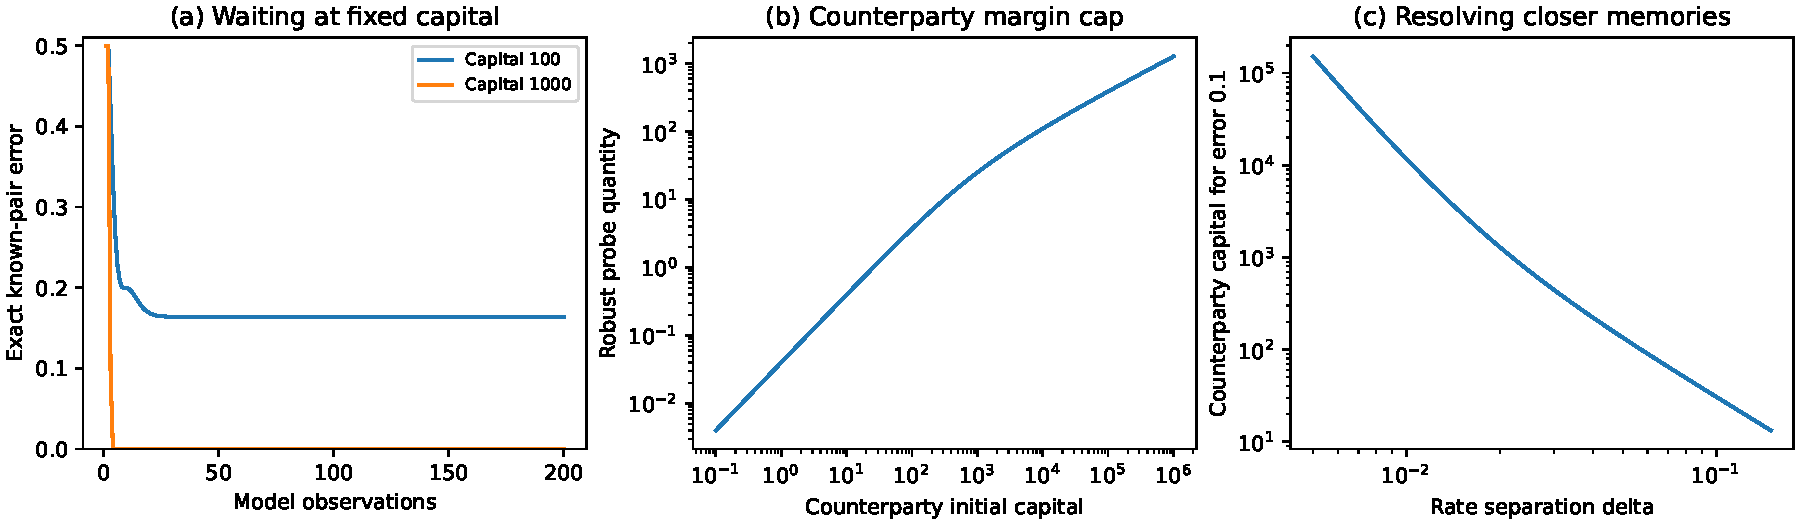
\includegraphics[width=\textwidth]{figures/fig_capital_information_20261008.pdf}
\caption{Constructed known-pair experiment funded by the counterparty cash/margin contract. Panel(a) gives exact Gaussian error at fixed counterparty capital 100 and 1,000, with separation0.05. Panel(b) gives the sharp robust quantity allowance. Panel(c) gives required capital within that counterparty quantity-ball contract for error 0.1 with 200 observations. Parameters are $a=0.5,\kappa=0.8,q=0.2,\eta=0.4$, observation SD 0.003, reference price100, margin 0.25 and cost 0.02. Quotes refresh after the uncontrolled update and executions pay half their direct impact. There is no process noise. These are imposed model units and fills. This plot does not give globally optimal probe-trader capital constants.}
\label{fig:capital_information}\end{figure*}

\begin{proposition}[Conditional Quote and Allocation Cost of Ambiguity]
\label{thm:welfare_opacity}
Consider a fixed one-unit ticket with monetary adverse mark $Z_\theta\sim N(\mu_\theta,\sigma_\theta^2)$ and a CARA dealer of risk aversion $\gamma>0$. Let $c_\theta=\mu_\theta+\gamma\sigma_\theta^2/2$ and suppose $c_\theta\ge0$ with $\sup_{\theta\in\Theta}c_\theta<\infty$. Under competition imposing zero robust certainty equivalent, the informed quote is $s_1=c_{\theta_0}$ and the ambiguous quote is $s_2=\sup_\theta c_\theta$ for $\theta_0\in\Theta$. Thus $\Delta=s_2-s_1\ge0$, with strict inequality precisely when the worst relevant cost exceeds $c_{\theta_0}$. Cohort nonidentification alone does not establish that condition or proportionality to a parameter diameter.

Under an additional allocation-surplus criterion with inverse demand $v(V)=(V_0-V)/b$ and fixed marginal cost $c$, raising an interior quote from $s_0$ to $s_0+\Delta$ produces surplus difference
\[
\mathcal W_{\rm loss}=b(s_0-c)\Delta+\frac b2\Delta^2.
\]
The triangle formula requires the efficient baseline $s_0=c$. Treating a risk charge as a social cost requires a defended welfare criterion.
\end{proposition}
\begin{proof}
Gaussian CARA certainty equivalent is $s-c_\theta$; its infimum is $s-\sup_\theta c_\theta$. The quote formulas follow from robust break-even. Equal costs throughout an observational equivalence class give zero premium. Integrating $v(V)-c$ between $V_0-b(s_0+\Delta)$ and $V_0-bs_0$ gives the stated surplus formula. Parameter coordinate rescaling can change a diameter while leaving costs and quotes unchanged.
\end{proof}

The set of relevant adverse-mark costs is an additional economic primitive; the aggregate cohort-equivalence theorem does not determine it. Likewise, a norm radius $B/\sup_\theta M_C(J_\theta)$ concerns a declared initial-state loss experiment and is not a quantity of posted depth. The empirical existence and magnitude of an ambiguity-induced liquidity or welfare effect remain open.


\subsection{Theorem 2: A Finite-Window Price-Surveillance Bound}
The following experiment isolates a statistical boundary under passive price observations. Its parameter $s$ is the scalar transition coefficient, distinct from the algebraic index $S=a+Q$ of a general multivariate market. Applying the result to a hidden multivariate market requires a valid observation-law reduction; no such reduction is inferred solely from a common unit-root boundary.

\begin{theorem}[Finite-Window Abstention in a Scalar Gaussian Experiment]
\label{thm:m3_minimax_abstention}
Observe $\mathcal D_T=(x_1,\ldots,x_T)$ where $x_0=0$ and $x_t=sx_{t-1}+w_t$, $w_t\sim\mathcal N(0,\sigma^2)$ independently, $\sigma>0$, and $s\in(0,2)$. Let a possibly randomized rule $\Psi$ take values Stable, Unstable, or Abstain, with
\[
\sup_{s<1}P_s(\Psi=\mathrm{Unstable})\le\alpha,
\qquad \sup_{s\ge1}P_s(\Psi=\mathrm{Stable})\le\alpha,
\quad 0<\alpha<1/2.
\]
Choose $0<c_0<1$ with $c_0e^{c_0}/(2\sqrt2)<1-2\alpha$. For every integer $T\ge1$, on $\mathcal B_T=(1-c_0/T,1+c_0/T)$,
\begin{equation}
\inf_{s\in\mathcal B_T}P_s(\Psi=\mathrm{Abstain})
\ge1-2\alpha-\frac{c_0e^{c_0}}{2\sqrt2}>0.
\label{eq:abstain_bound}
\end{equation}
For every finite $T$, the minimax worst-case error of binary rules across $s\in(0,2)$ is at least $1/2$.
\end{theorem}
\begin{proof}
Pair any $s_0\in(1-c_0/T,1)$ with $s_1=s_0+c_0/T\in(1,1+c_0/T)$; reverse the pairing for a point on the other side, including $s_1=1$. Gaussian transition densities give
\[
D_{\rm KL}(P_{s_0}\|P_{s_1})
=\frac{(s_1-s_0)^2}{2\sigma^2}\sum_{t=1}^T E_{s_0}x_{t-1}^2.
\]
For either paired coefficient, $|s|\le1+c_0/T$ and
$E_sx_{t-1}^2=\sigma^2\sum_{j=0}^{t-2}s^{2j}\le\sigma^2(t-1)e^{2c_0}$.
Thus the KL divergence in either direction is at most $c_0^2e^{2c_0}/4$ and Pinsker's inequality bounds total variation by $c_0e^{c_0}/(2\sqrt2)$. Error control gives $P_{s_0}(\mathrm{Unstable})\le\alpha$ and $P_{s_0}(\mathrm{Stable})\le P_{s_1}(\mathrm{Stable})+\mathrm{TV}\le\alpha+\mathrm{TV}$, yielding the stated abstention bound. The reverse pairing is identical.

For binary rules, the Gaussian path densities are continuous in $s$ in total variation at each finite $T$. Let $s^-\uparrow1$ and $s^+\downarrow1$. Le Cam's two-point bound gives worst-case error at least $(1-\|P_{s^-}-P_{s^+}\|_{\rm TV})/2\to1/2$. This is a worst-case statement over arbitrarily close alternatives; it is not a 50\% error claim at every fixed separated parameter.
\end{proof}

The theorem forces a positive probability of withholding a classification under the specified uniform error guarantee. It does not require abstention on every sample path. Initial conditions, extra measurements, and observation noise can change the inference problem. In particular, a fully observed noiseless cohort recursion need not admit the common Lebesgue densities assumed by an informal reduction to a scalar price likelihood. The exact-disclosure supplement gives a constructive two-step identification result under an exact single-cohort state/demand contract. Thus observing aggregate demand as well as the true price state can change the statistical experiment and defeat a universal extension of the scalar bound.


\begin{figure}[tbp]
\centering
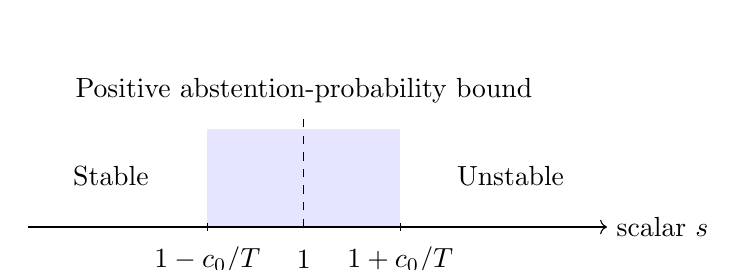
\begin{tikzpicture}[x=3.5cm,y=1cm]
\fill[blue!10] (-0.35,0) rectangle (0.35,1.25);
\draw[->] (-1,0)--(1.1,0) node[right]{scalar $s$};
\draw[dashed] (0,0)--(0,1.4);
\draw (-0.35,-0.05)--(-0.35,0.05) node[below=5pt]{$1-c_0/T$};
\draw (0.35,-0.05)--(0.35,0.05) node[below=5pt]{$1+c_0/T$};
\node[below=5pt] at (0,0){$1$};
\node at (-0.7,0.65){Stable};\node at (0.75,0.65){Unstable};
\node[above] at (0,1.45){Positive abstention-probability bound};
\end{tikzpicture}
\caption{Illustrative scalar Gaussian boundary under uniform error control. The shaded interval has a positive lower bound on abstention probability, rather than requiring every observed path to abstain. It is not a universal boundary for richer observation contracts.}
\label{fig:abstention_zone}
\end{figure}
\subsection{Financial Intermediary Solvency and Non-Normal Transient Amplification}
We now confront the fundamental divergence between price stability and financial intermediary solvency. In standard economic policy models, market stability is evaluated exclusively through the spectral radius $\rho(J) < 1$. We demonstrate that this criterion is dangerously incomplete.

\paragraph{The Non-Normal Market Jacobian.}
Consider the closed-loop Jacobian matrix $J$ from \eqref{eq:full_jacobian}. In financial markets, price impact and memory adaptation are asymmetric: order flow directly affects prices through contemporaneous impact $\kappa$, while price innovations affect memory through learning rate $\eta$. As a result, $J J^\top - J^\top J \neq 0$: the closed-loop market Jacobian $J$ is generically \textbf{non-normal} under asymmetric price-impact and learning parameters (except on a measure-zero algebraic subvariety). While normal matrices have orthogonal eigenvectors that diagonalize under unitary transformations, non-normal matrices have non-orthogonal (nearly parallel) eigenvectors. Consequently, even when all eigenvalues are strictly inside the unit circle ($|\lambda_i(J)| \le \rho(J) < 1$), matrix powers $J^t$ can undergo massive transient amplification before decaying asymptotically as $t \to \infty$ \citep{trefethen2005spectra}.

\paragraph{Optimizing Market Maker Problem and the Commitment Trap.}
To microfound the intermediary's financial vulnerability, we model a risk-averse, competitive market maker operating in continuous electronic order books \citep{ho1981optimal,grossman1988liquidity,avellaneda2008high,menkveld2013}. At each instant, the dealer quotes bid and ask prices (or an effective price-impact schedule $\kappa$ and half-spread $s_t$) to maximize expected inventory-adjusted fee revenue:
\begin{equation}
\max_{s_t, D_t} \mathbb{E}_t \left[ \sum_{k=0}^\infty \beta^k \left( s_{t+k} |q_{t+k}| - \frac{\phi}{2} I_{t+k}^2 \right) \right],
\label{eq:dealer_optimization}
\end{equation}
subject to inventory dynamics $I_{t+1} = I_t - q_t$, where $q_t$ is aggressive incoming order flow, $\phi > 0$ represents the inventory holding penalty, and $\beta \in (0, 1)$ is the discount factor. 

The market maker is subject to two institutional market design frictions:
\begin{enumerate}
    \item \textbf{Regulatory Capital and Margin Requirements:} The dealer maintains equity capital $E_t$ subject to a maximum regulatory leverage constraint or margin haircut $\mu \in (0, 1)$ on inventory positions: $\mu |I_t| p_t \le E_t$, with equity evolving as $E_{t+1} = E_t + \Pi_t$, where $\Pi_t = s_t |q_t| + (I_t-q_t)(p_{t+1}-p_t)-f_t-g_t$ is trading P\&L. Positive $q_t$ denotes a dealer sale at the current midpoint plus signed spread; $f_t,g_t$ are monetary fees and funding charges. This follows from cash $C_{t+1}=C_t+q_tp_t+s_t|q_t|-f_t-g_t$ and inventory $I_{t+1}=I_t-q_t$, marked at $p_{t+1}$.
    \item \textbf{Execution Latency and Affirmative Quoting Commitments:} Registered market makers face regulatory affirmative obligations (spread caps $\bar{s}$ and minimum depth commitments $\underline{D}$ required by exchange rules) and high-frequency cancellation latency $\tau_{\text{cancel}} > 0$. Once resting limit orders are posted in the order book, they remain committed for the cancellation latency window.
\end{enumerate}

The dynamic objective requires a demand/fill law and a financially specified continuation state before its optimal depth can be solved. The initial available monetary capital and a declared model loss budget satisfy
\begin{equation}
A_0=E_0-\mu|I_0|p_0,\qquad 0<B\le A_0.
\label{eq:dealer_buffer}
\end{equation}
This choice alone does not ensure future margin feasibility. The former division by $1+\phi/\mu$ lacked a unit-consistent shadow-cost derivation.

\begin{lemma}[Conditional Capacity Choice and Depth-Dependent Stability]
\label{lem:endogenous_kappa}
For a static capacity illustration, fix net execution edge $r\ge0$, holding coefficient $h>0$, capital per quantity $m>0$, and bounds $L_{\min}\le L\le L_{\max}$. Maximize $rL-hL^2/2$ subject to $mL\le A$. If $\bar L=\min(L_{\max},A/m)<L_{\min}$, the quoting commitment is infeasible. Otherwise
\begin{equation}
L^*=\min\{\bar L,\max(L_{\min},r/h)\},\qquad
D^*=L^*/w,\quad \kappa^*=w/L^*\quad(L^*>0),
\label{eq:endogenous_kappa}
\end{equation}
where $w>0$ is a declared linear-book price width. Capital raises capacity weakly; nonbinding capital changes leave capacity unchanged. This is a solved one-period illustration with fixed primitives, rather than a solution of the preceding dynamic dealer objective.

For one cohort, fixed $\varphi>0$ and $0<\eta<1$, substituting $a=1-\kappa\varphi$ into the cohort transition gives Schur stability precisely when
\[
q<\varphi,\qquad
0<\kappa<\frac{4-2\eta}{(2-\eta)\varphi-\eta q}.
\]
Higher impact changes both persistence and coupling and does not necessarily increase transient magnification.
\end{lemma}
\begin{proof}
Strict concavity gives the unconstrained optimum $r/h$; projection onto the feasible interval gives $L^*$. The depth/impact relation is the declared clearing schedule. The three Jury quantities are $\kappa\eta(\varphi-q)$, $4-2\eta-\kappa[(2-\eta)\varphi-\eta q]$, and $\eta+(1-\eta)\kappa\varphi$, which yield the stated stability conditions.

For an exact counterexample, fix $\varphi=1,q=1/10,\eta=9/10$. At $\kappa=1/10$, the first column of $J$ is $(9/10,81/100)^\top$ and its squared norm is $14661/10000>1$. At $\kappa=1$, $J=\left(\begin{smallmatrix}0&1/10\\0&19/100\end{smallmatrix}\right)$ has squared operator norm $461/10000<1$. Both are stable. In the fixed all-state Euclidean experiment, the former has peak magnification greater than one, while the latter has peak one. Thus increasing impact can reduce transient risk in the stated model.
\end{proof}

\textbf{The Solvency Trap:} Why doesn't the optimizing dealer step away or widen spreads before non-normal amplification hits? Doing so violates exchange affirmative obligations (risking forfeiture of market-maker status and exchange fee rebates) or cedes order flow to Bertrand competitors. Furthermore, when an aggressive algorithmic feedback cascade arrives within the cancellation window $\tau_{\text{cancel}}$, resting passive limit orders are executed against at stale quotes before the dealer can cancel or widen spreads \citep{budish2015}. The following theorem concerns a declared model loss output $\ell_t=Cz_t$, $z_t=J^tz_0$, with $C$ in the same monetary budget units as $B$. Actual cash, post-trade inventory, prices, fees, funding and margin changes must justify that output mapping. It does not follow from setting inventory equal to a latent-state norm. The model loss-budget breach is $\sup_{t\ge0}|CJ^tz_0|>B$; operational solvency requires the additional accounting contract.

\begin{theorem}[Conditional Loss Budget and Kreiss Bounds]
\label{thm:m5_kreiss_solvency}
Let $z_t = J^t z_0$ with $\rho(J) < 1$, balance-sheet buffer $B > 0$, and observation matrix $C$.
\begin{enumerate}
    \item \textbf{Exact Worst-Case Safe Radius:} For the declared criterion $\sup_t\|CJ^tz_0\|_2\le B$, the exact maximum initial-state radius is:
    \begin{equation}
    r^*_{\text{exact}} = \frac{B}{\sup_{t \ge 0} \|C J^t\|_2} \equiv \frac{B}{M_C},
    \label{eq:exact_safe_radius}
    \end{equation}
    where $M_C \equiv \sup_{t \ge 0} \|C J^t\|_2$ is the declared output gain. If $C=0$, the allowance is unbounded by this criterion; actual financial constraints still apply.
    \item \textbf{Kreiss Lower and Upper Bounds:} Under full state observation ($C = I$), the Kreiss constant of matrix $J$, defined on the resolvent outside the unit disk:
    \begin{equation}
    \mathcal{K}(J) \equiv \sup_{|z| > 1} (|z| - 1) \|(zI - J)^{-1}\|_2,
    \label{eq:kreiss_def}
    \end{equation}
    satisfies $\mathcal{K}(J) \le \sup_{t \ge 0} \|J^t\|_2 \le e \cdot n \cdot \mathcal{K}(J)$ for any $J \in \R^{n \times n}$. Consequently:
    \begin{equation}
    r_{\text{conservative}} \equiv \frac{B}{e \cdot n \cdot \mathcal{K}(J)} \le r^*_{\text{exact}} \le \frac{B}{\mathcal{K}(J)}.
    \label{eq:kreiss_bilateral_bound}
    \end{equation}
    \item \textbf{Complete Failure of Spectral Radius:} For any stable spectral radius $\rho \in (0, 1)$ and any arbitrarily small buffer $B > 0$, there exists a parameter family of non-normal matrices $J_\theta$ and an observation operator $C = [1, 0]$ exposed to the amplified coordinate such that $\rho(J_\theta) = \rho$ for all $\theta$, while the exact safe radius collapses to zero:
    \begin{equation}
    \lim_{\theta \to \infty} r^*_{\text{exact}}(J_\theta) = 0.
    \end{equation}
\end{enumerate}
\end{theorem}

\begin{proof}[Proof Sketch]
Part~1 follows from the Cauchy--Schwarz inequality for operator norms: maximum loss across $\|z_0\|_2 \le r$ is $r \cdot \sup_{t \ge 0} \|C J^t\|_2 = r M_C$, yielding $r^*_{\text{exact}} = B/M_C$. Part~2 applies Spijker's (1991) optimal resolution of the Kreiss matrix conjecture, establishing $\mathcal{K}(J) \le \sup_{t \ge 0} \|J^t\|_2 \le e \cdot n \cdot \mathcal{K}(J)$ for $C=I$. Part~3 uses $J_\theta=\left(\begin{smallmatrix}\rho&\theta\\0&\rho\end{smallmatrix}\right)$. Then $CJ_\theta=(\rho,\theta)$, so $M_C\ge\sqrt{\rho^2+\theta^2}\to\infty$. The family is defective; no eigenvector-basis argument is required.
\end{proof}

\begin{remark}[Output and disturbance geometry]
The theorem applies to a specified initial-state ball and output norm. State coordinate changes require a corresponding change in the disturbance set; arbitrary latent-state units cannot be interpreted as monetary losses. A physical execution-input experiment has a different gain, as Theorem~\ref{thm:resource_frontier} shows. The Kreiss lower radius concerns full-state observation. A small spectral radius alone supplies no universal bound, but non-normality alone does not establish severe monetary losses in a calibrated market.
\end{remark}

\subsection{Pseudospectral Contours and Non-Normal Resolvent Bounds}
To gain deeper visual and geometric intuition into why the spectral radius fails to predict dealer solvency, we examine the $\epsilon$-pseudospectrum of the closed-loop market Jacobian. For any $\epsilon > 0$, the $\epsilon$-pseudospectrum $\sigma_\epsilon(J)$ of matrix $J$ is defined as the set of complex numbers $z \in \mathbb{C}$ satisfying:
\begin{equation}
\sigma_\epsilon(J) \equiv \left\{ z \in \mathbb{C} : \|(zI - J)^{-1}\|_2 \ge \epsilon^{-1} \right\}.
\label{eq:pseudospectrum_def}
\end{equation}
Equivalently, $\sigma_\epsilon(J)$ represents the union of all eigenvalues of perturbed matrices $J + E$ across all perturbations with $\|E\|_2 \le \epsilon$.

As visualized in Figure~\ref{fig:pseudospectrum}, in a normal system, the pseudospectrum consists of concentric disks of radius $\epsilon$ centered at the eigenvalues: $\sigma_\epsilon(J) = \bigcup_i \{z : |z - \lambda_i| \le \epsilon\}$. However, for a constructed non-normal matrix, computed pseudospectral contours can stretch along the off-diagonal coupling direction, protruding significantly outside the unit circle $\{|z| = 1\}$ even when the spectral radius $\rho(J) = 0.50$ is well within the interior. 

The Kreiss constant $\mathcal{K}(J)$ measures the maximum ratio by which these pseudospectral contours protrude beyond the unit circle:
\begin{equation}
\mathcal{K}(J) = \sup_{\epsilon > 0} \frac{\alpha_\epsilon(J) - 1}{\epsilon}, \qquad \alpha_\epsilon(J) \equiv \sup_{z \in \sigma_\epsilon(J)} |z|.
\end{equation}
Whenever $\mathcal{K}(J) \gg 1$, small high-frequency liquidity shocks are magnified by the non-normal resolvent, inducing large transient balance-sheet losses that exhaust dealer margin buffers before eigenvalue decay can assert itself.

\begin{figure}[tbp]\centering
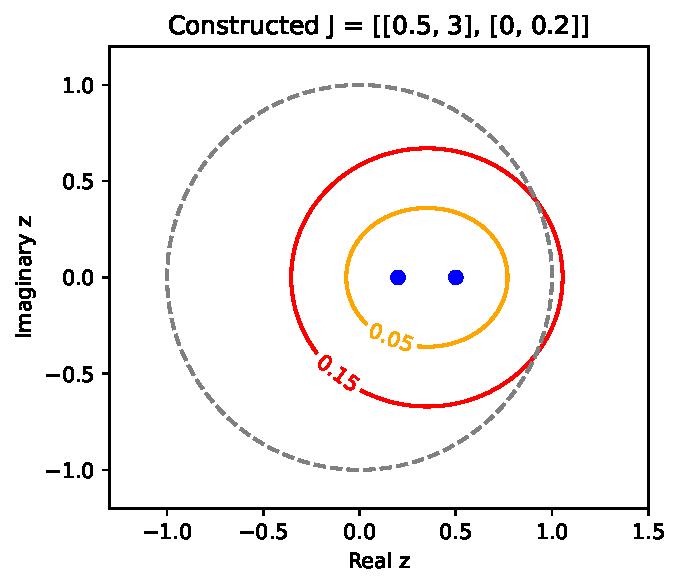
\includegraphics[width=0.65\textwidth]{figures/fig_verified_pseudospectrum_20261008.pdf}
\caption{Computed singular-value contours for the declared constructed matrix $J=\left(\begin{smallmatrix}0.5&3\\0&0.2\end{smallmatrix}\right)$ at 0.05 and 0.15. Its spectral radius is 0.5; the 0.15 contour crosses the unit circle. This fixed-coordinate illustration is not a calibrated cohort-market or monetary-loss experiment.}
\label{fig:pseudospectrum}\end{figure}

\subsection{Multi-Asset Generalization and Cross-Impact Kreiss Inflation}
Modern market makers operate simultaneously across multiple correlated instruments (e.g., BTC, ETH, and altcoins; or equity index components and ETFs). In multi-asset environments, cross-asset price impact creates additional non-normal coupling.

Let $\mathbf{x}_t \in \R^d$ denote the vector of pricing errors across $d$ traded assets, and let $\mathbf{u}_t \in \R^d$ denote aggregate order flows. The multi-asset price formation equation is:
\begin{equation}
\mathbf{x}_{t+1} = \mathbf{A} \mathbf{x}_t + \mathbf{K} \mathbf{u}_t + \mathbf{w}_{t+1},
\label{eq:multi_price}
\end{equation}
where $\mathbf{A} = \diag(a_1, \dots, a_d) \in \R^{d \times d}$ collects direct price persistences, and $\mathbf{K} \in \R^{d \times d}$ is the cross-asset price impact matrix. For the following mathematical feedforward benchmark, allow $\mathbf K$ to be asymmetric. No causal instantaneous cross-asset impact matrix is calibrated here. A transactional interpretation additionally requires an execution-cost law consistent with no-price-manipulation restrictions; cross-impact symmetry under the relevant bounded-kernel assumptions is a substantive economic constraint \citep{schneiderlillo2017}.

Each asset is traded by adaptive momentum flow with learning rates $\mathbf{H} = \diag(\eta_1, \dots, \eta_d)$ and feedback gain $\mathbf{Q} \in \R^{d \times d}$:
\begin{equation}
\mathbf{y}_{t+1} = (\mathbf{I} - \mathbf{H}) \mathbf{y}_t + \mathbf{H} \mathbf{x}_{t+1}, \qquad \mathbf{u}_t = \mathbf{Q} \mathbf{y}_t.
\end{equation}
Stacking $\mathbf{z}_t = (\mathbf{x}_t^\top, \mathbf{y}_t^\top)^\top \in \R^{2d}$, the multi-asset closed-loop Jacobian is:
\begin{equation}
J_{\text{multi}} = \begin{bmatrix}
\mathbf{A} & \mathbf{K} \mathbf{Q} \\
\mathbf{H} \mathbf{A} & \mathbf{I} - \mathbf{H} + \mathbf{H} \mathbf{K} \mathbf{Q}
\end{bmatrix} \in \R^{2d \times 2d}.
\label{eq:multi_jacobian}
\end{equation}

\begin{proposition}[Cross-Impact Kreiss Inflation and Safe Radius Bound in Directed Networks]
\label{prop:cross_kreiss}
Consider a multi-asset economy with directed block-triangular leader-satellite cross-impact ($K_{12} = 0, K_{21} > 0$), diagonal feedback matrices $\mathbf{Q} \ge 0$, anchor matrices $\mathbf{A} \ge 0$, adaptation rates $\mathbf{H} \in (0, 1)^d$, nonnegative impact matrix $\mathbf K\ge0$, stable diagonal blocks, and fixed output operator $C\ge0$. Let $J_{\text{diag}}$ denote the decoupled Jacobian where $K_{21} = 0$.
The directed coupling introduces off-diagonal block feedforward, inflating the Kreiss constant: $\mathcal{K}(J_{\text{multi}}) \ge \mathcal{K}(J_{\text{diag}})$. Consequently, the Kreiss-based conservative safe radius bound contracts: $r_{\text{conservative}}(J_{\text{multi}}) \equiv \frac{B}{e (2d) \mathcal{K}(J_{\text{multi}})} \le r_{\text{conservative}}(J_{\text{diag}})$.
For the exact safe shock radius $r^*_{\text{exact}}(J) \equiv B / M_C(J)$, because all constituent blocks of $J$ are entrywise non-negative in the momentum economy, matrix powers $J_{\text{multi}}^t$ are entrywise non-decreasing in $K_{21}$, yielding $M_C(J_{\text{multi}}) \ge M_C(J_{\text{diag}})$ and exact radius contraction $r^*_{\text{exact}}(J_{\text{multi}}) \le r^*_{\text{exact}}(J_{\text{diag}})$. A fixed-coordinate constructed coupling can increase peak gain. Its magnitude requires a declared output and shock set; no empirical percentage follows from this proposition.
\end{proposition}
\begin{proof}
Permute coordinates by asset; directed impact makes the full transition block triangular, preserving the stable diagonal spectra. Entrywise $0\le J_{diag}\le J_{multi}$ implies ordered nonnegative powers and ordered Euclidean operator norms after multiplication by fixed nonnegative $C$. For $r>1$, the nonnegative Neumann series $(rI-J)^{-1}=\sum_{t\ge0}J^t/r^{t+1}$ is likewise ordered. At any complex $z$ with $|z|=r$, its modulus is entrywise bounded by this real-radius resolvent, so the norm supremum on that circle occurs at $z=r$. Taking the Kreiss supremum proves its monotonicity. The statements concern fixed coordinates and nonnegative output; signed hedge outputs need separate analysis.
\end{proof}


Proposition~\ref{prop:cross_kreiss} concerns nonnegative downstream coupling under fixed shock/output geometry. Hedged or signed monetary outputs need separate treatment; they do not inherit a universal monotonic radius comparison. The earlier empirical 14.5-percent calibration claim is not established by this proof.

\section{Data and Empirical Identification Strategy}
\label{sec:data_estimand}

\subsection{Econometric Estimand and Moving-Average Filtering}
We compute reduced-form indices under explicit price/flow constructions. Their algebra is invariant to consistent constant price and flow rescaling, but this does not identify structural learning or physical execution impact.

A fundamental gap between theoretical models and high-frequency empirical execution concerns the definition of the state variable. In theoretical models (Section~\ref{sec:model}), $x_t \equiv p_t - p_t^*$ represents price displacement relative to an unobserved fundamental value $p_t^*$. In empirical limit order books, true fundamental value is unobservable, and econometricians routinely replace $p_t^*$ with a trailing price filter, such as an Exponential Moving Average (EMA).

Let $p_b$ denote a log recorded-price proxy sampled at discrete uniform time bars $b$ of length $\Delta$ (e.g., $\Delta = 10$~seconds). The trailing exponential moving-average anchor $m_b$ is defined by the recursive filter:
\begin{equation}
m_b = (1 - \alpha) m_{b-1} + \alpha p_b, \qquad \alpha \equiv \frac{2}{W/\Delta + 1},
\label{eq:ema_def}
\end{equation}
where the proxy is transaction close for Binance trade bars and midpoint for the recorder. Multiplication of log prices by 10,000 changes their units, not the stated constant-scaling invariants. Here $W$ is the smoothing window (e.g., $W = 300$~seconds, yielding $\alpha = 2/31 \approx 0.064516$). The empirical state variable is defined as the deviation from this trailing anchor:
\begin{equation}
x_b^{\text{EMA}} \equiv p_b - m_b = (1 - \alpha)(p_b - m_{b-1}) = \frac{1 - \alpha}{1 - (1 - \alpha) L} \Delta p_b.
\label{eq:x_ema_rep}
\end{equation}

\begin{proposition}[Mechanical Persistence under Filtered Random Walks]
\label{prop:mechanical_persistence}
Suppose the log mid-price $p_b$ follows an unpredictable martingale (random walk), such that $\mathbb{E}[p_{b+1} \mid \mathcal{F}_b] = p_b$. Then the moving-average deviation state $x_b^{\text{EMA}}$ mechanically follows an autoregressive AR(1) process:
\begin{equation}
\mathbb{E}[x_{b+1}^{\text{EMA}} \mid \mathcal{F}_b] = (1 - \alpha) x_b^{\text{EMA}},
\label{eq:mechanical_ar1}
\end{equation}
with mechanical persistence parameter $a_0 \equiv 1 - \alpha = \frac{29}{31} \approx 0.93548$.
\end{proposition}

\begin{proof}
By definition, $x_{b+1}^{\text{EMA}} = p_{b+1} - m_{b+1} = (1 - \alpha)(p_{b+1} - m_b)$. Conditioning on information $\mathcal{F}_b$:
\begin{equation}
\mathbb{E}[x_{b+1}^{\text{EMA}} \mid \mathcal{F}_b] = (1 - \alpha) \left( \mathbb{E}[p_{b+1} \mid \mathcal{F}_b] - m_b \right) = (1 - \alpha)(p_b - m_b) = (1 - \alpha) x_b^{\text{EMA}},
\end{equation}
which establishes \eqref{eq:mechanical_ar1} with mechanical persistence $a_0 = 1 - \alpha$.
\end{proof}

\begin{remark}[Economic Interpretation of Empirical Feedback $\hat Q$]
The EMA state measures deviation from a trailing price proxy rather than the unobserved fundamental value. In the corrected observed-flow panel, equal-weight pooled date means give $\hat Q=0.0003807$ and $\hat S=0.9203825$, hence the corresponding mean $\hat J_{11}=0.9200018$. The mechanical martingale anchor is $29/31\simeq0.9354839$ for this filter. A smaller fitted coefficient is a descriptive comparison; it does not prove market-level fundamental stability, identify bid--ask bounce or inventory replenishment as its cause, or authenticate a structural feedback mechanism.
\end{remark}

Let $f_t$ denote the sample-specific flow feature. Binance uses notional taker buy volume minus taker sell volume over the observed bar; recorder features and quote OFI use the separately declared constructions. The empirical bivariate vector autoregressive (VAR(1)) representation of joint price-flow transitions is:
\begin{equation}
\begin{bmatrix} x_{t+1}^{\text{EMA}} \\ f_{t+1} \end{bmatrix} = \begin{bmatrix} J_{11} & J_{12} \\ J_{21} & J_{22} \end{bmatrix} \begin{bmatrix} x_t^{\text{EMA}} \\ f_t \end{bmatrix} + \begin{bmatrix} e_{1, t+1} \\ e_{2, t+1} \end{bmatrix}, \qquad \E[\mathbf{e}_t \mathbf{e}_t^\top] = \Sigma_e,
\label{eq:bivariate_var}
\end{equation}
Here all $J_{ij}$ are reduced-form coefficients for the constructed state and flow. They are not authenticated physical impact or latent learner parameters. When its denominators are nonzero, we extract dimensionless invariants $\hat{Q} \equiv \frac{\hat{J}_{12} \hat{J}_{21}}{1 - \hat{J}_{22}}$, $\hat{S} \equiv \hat{J}_{11} + \hat{Q}$, and $\hat{\mathcal{L}} \equiv \frac{\hat{Q}}{1 - \hat{J}_{11}}$, which are strictly scale-invariant.

\subsection{Measurement Sensitivity: How Clocks and Filters Dominate Feedback}
\label{sec:measurement_sensitivity}
Table~\ref{tab:measurement_sensitivity} reconstructs the measurement comparison from the existing BTC, ETH and ADA recorder caches. One-second records are aggregated into ten-second bins, with a 300-second trailing EMA. The preserved filter resets at gaps and continues across contiguous UTC dates; regressions and lags split at gaps and dates. This is a recorded-series diagnostic. Exact primary-source byte matching and uploader-declared CC0 are documented below; the economic interpretation of its recorded flow remains a separate question.

\begin{table}[htbp]
\centering\footnotesize
\setlength{\tabcolsep}{3pt}
\caption{Reconstructed recorded-series timing/state diagnostics. Mean $Q$ and exploratory date-level Student intervals are based on 13 sampled dates; serial independence and universal coverage are not established. All three assets and constructions are retained.}
\label{tab:measurement_sensitivity}
\begin{tabular}{llrrrl}\toprule
Asset & State / clock & Dates & Transitions & Mean $Q$ & Date interval \\\midrule
BTC & EMA / observed & 13 & 102470 & 0.0019353 & [0.00032, 0.00355] \\
BTC & EMA / forward & 13 & 102454 & 0.0125227 & [0.00653, 0.01851] \\
BTC & Return / observed & 13 & 102470 & 0.0012059 & [-0.00067, 0.00308] \\
ETH & EMA / observed & 13 & 102771 & 0.0009795 & [0.00006, 0.00190] \\
ETH & EMA / forward & 13 & 102757 & 0.0113018 & [0.00806, 0.01454] \\
ETH & Return / observed & 13 & 102771 & 0.0003310 & [-0.00035, 0.00101] \\
ADA & EMA / observed & 13 & 102898 & 0.0006163 & [0.00016, 0.00108] \\
ADA & EMA / forward & 13 & 102885 & 0.0072058 & [0.00564, 0.00877] \\
ADA & Return / observed & 13 & 102898 & 0.0000018 & [-0.00094, 0.00094] \\
\bottomrule\end{tabular}
\end{table}

The forward variant pairs the price state $x_b$ with next-bin flow $F_{b+1}$ rather than observed $F_b$, creating look-ahead information in the state pairing. It is not a separately authenticated future 60-second execution window. The raw-return date intervals include zero for all three assets. The baseline recorder construction admits 75, 72 and 69 partial bins for BTC, ETH and ADA. A stricter sensitivity requires ten observed seconds and resets the EMA across resulting gaps: mean observed-EMA $Q$ becomes 0.0010800, 0.0007072 and 0.0004148. Its ADA EMA interval spans zero; all three strict raw-return intervals also span zero. Every strict sample count, date estimate and interval is retained. The baseline covariance, switching and shuffle studies refer to their explicitly retained occupied-bin construction, rather than claiming complete-bin robustness. These results establish sensitivity to the declared timing and state construction; non-rejection does not establish absent learning or a universal explanation of market behavior. The earlier narrow HAC intervals, raw-return literals and SOL recorder label are not authenticated by these calculations and are replaced by the named result fields.

\paragraph{Controlling for Order-Splitting Memory.}
The diagnostic \[Q_L=\hat J_{12}\hat c_L/(1-\sum_{\ell=1}^L\hat\phi_\ell)\] uses the regression $F_{b+1}$ on $x_b,F_b,\ldots,F_{b-L+1}$. Here $L$ counts bars, not seconds, and $L=1$ recovers VAR(1). This is an observable long-run response functional; omitted fundamentals, endogenous flow, near-zero denominators and filtering can prevent a structural interpretation.

\subsection{Covariance Restrictions and the Limits of Heteroskedastic Identification}
For a stationary VAR, $\Gamma_0=J\Gamma_0J^\top+\Sigma$ and $\Gamma_k=J^k\Gamma_0$. Matching three contemporaneous and eight lagged covariance entries gives 11 moments and seven transition/noise parameters. Our diagnostic uses a full stable transition and positive-definite innovation parameterization, segment-aware moment HAC and six starts per declared case. All 24 cases (three assets, two centering rules and four bandwidths) reject their maintained restrictions under their stated asymptotic reference. For global centering and bandwidth ten bars, $J$ statistics are 41.4063, 28.3094 and 12.1175 for BTC, ETH and ADA. These rejections do not validate the fitted economic model. The earlier restricted-fit statistic 73 concerns a different parameter class and is retained only in the historical ledger.

Contemporaneous heteroskedastic identification additionally requires invariant structural coefficients, valid innovations, orthogonal structural shocks and a defended regime partition. Nonproportional variance shifts alone do not supply all of these. In the two-equation system, exchanging shock labels maps $(\lambda,c)$ to $(1/c,1/\lambda)$ while preserving each covariance after variance rescaling. Sign or economic exclusions can distinguish some branches, but the current source's single bounded numerical root is not an identification proof. Its forward-flow pairing and endogenous volatility grouping do not establish the required assumptions. Thus the old negative coefficient is not evidence that market makers provide identified instantaneous buffering. The exact branch-equivalence witness and all covariance sensitivities are retained.

\subsection{Data Coverage, Representation and Authentication}
The supplied data are different measurement objects. Official Binance trade bars have raw executed-volume fields; the recorder files contain supplied quote/flow features; the equity representation is event-indexed; the January file contains depth snapshots. Counts of these objects cannot be combined into a count of independent, continuous one-second transitions. The three recorder CSVs match the Nielsen version 1 provider release byte for byte, with provider archive CRC and full SHA256 checks. Its primary metadata declares CC0. The FI-2010 primary metadata declares CC BY 4.0; the local mirror licence does not supersede it. Its supplied transformation has been exactly replayed against independently retrieved normalized files; primary-archive hash, local company-label mapping and reconstructed physical scales remain unauthenticated. Current Binance Vision terms specify CC BY-NC-SA 4.0 for the downloaded data; the final derivative-release package must reflect the provider terms. The January CSV now also matches the original siavashraz version 1 CSV byte for byte (uploader-declared MIT). That provider describes Binance Bitcoin perpetual BTCUSDT.P data at nominal 250-millisecond sampling. The separately matched szh765 Parquet distribution declares Apache 2.0. These establish distribution identity and provider-declared venue/contract, rather than independent exchange authentication. Source metadata, hashes and licence texts accompany this revision. 
\begin{table}[htbp]
\centering\footnotesize\setlength{\tabcolsep}{3pt}
\caption{Exact working-sample coverage. Original-provider attribution and reuse permission are separate from local file hashes.}
\label{tab:datasets}
\begin{tabularx}{\textwidth}{lXXX}\toprule
Sample & Coverage & Raw rows / representation & Source status \\\midrule
Binance spot & 96 dates, 2021--2024 & 66,316,704 one-second bar rows & Current official checksums \\
Recorded BTC/ETH/ADA & April 7--19, 2021 & Existing second-indexed feature files & Primary version 1 bytes matched \\
Supplied equity & 50 legacy labels; 49 legacy fits & 272,941 event snapshots & Mirror replay matched; mapping open \\
January BTC depth & January 9--20, 2023 & 3,730,870 raw snapshots & Primary distribution matched \\
\bottomrule\end{tabularx}
\end{table}

The Binance reconstruction retains the first duplicate timestamp and requires all ten observed seconds per primary bar. It resets the EMA at each gap and date, burns 150 ten-second states and estimates sufficiently long segments separately. There are 38,859 missing seconds and 363 duplicate seconds across the reconstructed study units, without conflicting duplicate rows. Legacy filling is reproduced solely to explain the original outputs. The recorder baseline admits occupied ten-second bins, including partial bins; its EMA resets at missing whole bins and continues across contiguous dates, while regressions split dates and those bin gaps. Consecutively repeated feature renders have their recorded flow set to zero under the archived deduplication rule; this reconstructs the cache but does not authenticate the underlying execution window. No universal winsorization or quote-filter percentage is asserted.

For quote OFI, a price increase contributes new bid size and a bid-price decrease removes old bid size; an unchanged bid contributes its size change. Ask signs reverse. Quote OFI is distinct from executed signed flow. The previous simplified price-indicator formula and claim that a depth proxy automatically purges endogeneity are not used.

\section{Original Panel and Fee-Schedule Comparison}
\label{sec:baseline_natural_exp}
\subsection{Baseline Reconstruction and Cross-Asset Measurement}
\begin{table}[htbp]
\centering\footnotesize\setlength{\tabcolsep}{3pt}
\caption{Original-panel measurement reconstruction: equal-weight means across assets within each of 96 sampled dates, followed by date means and exploratory Student intervals. The 768 study units contain 66,316,704 raw one-second rows; primary fits use 6,513,239 ten-second transitions. These are reduced-form diagnostics.}
\label{tab:binance_panel}
\resizebox{\textwidth}{!}{\begin{tabular}{lrrrrr}\toprule
Construction & $Q$ & Date interval & $S$ & Date interval & $Q>0$ share \\\midrule
Legacy forward-flow & 0.0081536 & [0.0072958, 0.0090114] & 0.9205544 & [0.9164297, 0.9246791] & 86.85\% \\
Observed-flow EMA & 0.0003807 & [0.0002412, 0.0005201] & 0.9203825 & [0.9160228, 0.9247423] & 62.37\% \\
Observed raw return & -0.0001625 & [-0.0003836, 0.0000585] & -0.0414724 & [-0.0517954, -0.0311494] & 48.83\% \\
\bottomrule\end{tabular}}
\end{table}
\begin{table}[htbp]
\centering\footnotesize\setlength{\tabcolsep}{3pt}
\caption{Original-panel asset means under explicit timing/state choices. $Q_{30}$ controls 30 ten-second bars (300 seconds); it is a long-run regression diagnostic. No participant or regulatory causal effect is identified.}
\label{tab:cross_asset_panel}
\resizebox{\textwidth}{!}{\begin{tabular}{lrrrrrr}\toprule
Pair & Days & Legacy $Q$ & Observed $Q$ & $Q_{30}$ & Return $Q$ & Observed $S$ \\\midrule
BTC/USDT & 96 & 0.0142386 & 0.0006350 & 0.0005751 & 0.0000594 & 0.9346384 \\
ETH/USDT & 96 & 0.0131252 & 0.0005657 & 0.0003358 & -0.0005013 & 0.9349149 \\
SOL/USDT & 96 & 0.0087132 & 0.0002036 & 0.0001314 & -0.0005210 & 0.9190796 \\
ADA/USDT & 96 & 0.0067986 & 0.0003953 & 0.0003623 & 0.0000840 & 0.9142432 \\
DOGE/USDT & 96 & 0.0059319 & 0.0002511 & 0.0001622 & -0.0002345 & 0.9245799 \\
BNB/USDT & 96 & 0.0057950 & 0.0004587 & 0.0002731 & -0.0000789 & 0.8946552 \\
XRP/USDT & 96 & 0.0057009 & 0.0002292 & 0.0001741 & -0.0004279 & 0.9233588 \\
LTC/USDT & 96 & 0.0049256 & 0.0003068 & 0.0002650 & 0.0003200 & 0.9175903 \\
\bottomrule\end{tabular}}
\end{table}

The original panel is fully reconstructed at its 768 named study units using current official archives. Calendar Bartlett HAC sensitivity at 30, 90, 180 and 365-day bandwidths retains positive pooled observed-EMA reference intervals and raw-return intervals spanning zero. These retrospective Gaussian references require additional mixing/stationarity assumptions; they do not establish causal or finite-sample coverage. All 32 index/measurement references accompany the revision. The large legacy positive estimate changes materially under observed-flow alignment; raw-return date intervals include zero for the pooled diagnostic. This is a measurement result, not a proof that learning is absent. A stable fitted VAR or $S<1$ is not an authenticated structural stability statement about the market.
\begin{figure*}[htbp]\centering
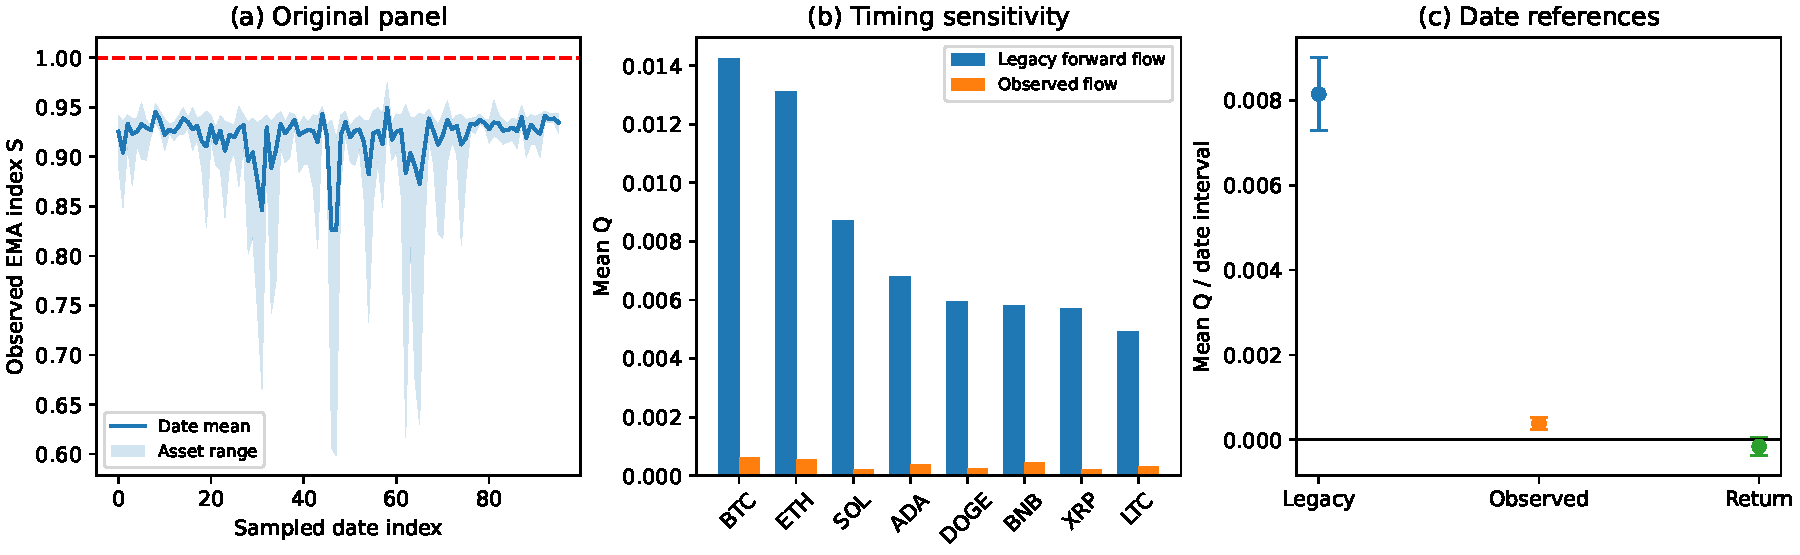
\includegraphics[width=\textwidth]{figures/fig_verified_panel_20261008.pdf}
\caption{Reconstructed original panel: observed EMA index by date, legacy versus observed asset means, and pooled date-level uncertainty for three measurement constructions. Every panel uses the raw-reproduced study units. No identified market-maker buffering coefficient is plotted.}
\label{fig:binance_panel_and_identification}\end{figure*}

\subsection{July 2022 Fee-Schedule Comparison and Inference}
For the 24 sampled 2022 dates, fit \[Y_{it}=\beta_0+\beta_1\mathrm{BTC}_i+\beta_2\mathrm{Post}_t+\beta_3\mathrm{BTC}_i\mathrm{Post}_t+e_{it}.\] Here post means dates on/after July 8. There are 192 rows and one treated asset. The reconstructed sampled-date mean BTC quote volume increases by 75.010858 percent; that descriptive difference is not a fee-induced causal estimate. Table~\ref{tab:natural_experiment_did} separates the actual covariance references instead of calling classical uncertainty clustered.
\begin{table}[htbp]
\centering\footnotesize\setlength{\tabcolsep}{3pt}
\caption{Recomputed BTC-by-post association in the original 192-unit 2022 panel. The same four-regressor specification is evaluated under three covariance references; cluster counts are eight assets and 24 sampled dates. The assignment is not randomized.}
\label{tab:natural_experiment_did}
\resizebox{\textwidth}{!}{\begin{tabular}{lrrrrrr}\toprule
State & Index & Reference & $\hat\beta_3$ & SE & df & $p$ \\\midrule
Legacy & Q & classical & -0.0018555 & 0.0030720 & 188 & 0.546569 \\
Legacy & Q & asset\ cluster & -0.0018555 & 0.0008841 & 7 & 0.074018 \\
Legacy & Q & date\ cluster & -0.0018555 & 0.0034116 & 23 & 0.591756 \\
Legacy & S & classical & -0.0003897 & 0.0245851 & 188 & 0.987370 \\
Legacy & S & asset\ cluster & -0.0003897 & 0.0195257 & 7 & 0.984634 \\
Legacy & S & date\ cluster & -0.0003897 & 0.0132341 & 23 & 0.976763 \\
Observed & Q & classical & -0.0001057 & 0.0004038 & 188 & 0.793794 \\
Observed & Q & asset\ cluster & -0.0001057 & 0.0002139 & 7 & 0.636344 \\
Observed & Q & date\ cluster & -0.0001057 & 0.0004449 & 23 & 0.814284 \\
Observed & S & classical & -0.0036464 & 0.0254227 & 188 & 0.886102 \\
Observed & S & asset\ cluster & -0.0036464 & 0.0203732 & 7 & 0.863022 \\
Observed & S & date\ cluster & -0.0036464 & 0.0140420 & 23 & 0.797420 \\
\bottomrule\end{tabular}}
\end{table}

For observed $Q$, the date-cluster interval is $[-0.001025969,0.000814559]$. Neither a non-rejection nor the cross-asset placebo ranking proves invariance or a parallel counterfactual. The old equivalence margin 0.007 is about 18 times the corrected pooled baseline; passing such a margin cannot establish economically meaningful equivalence. Asset comparisons are not random treatment reassignments. Serial dependence across sampled dates, spillovers and the single treated unit remain material inference limitations.
\subsection{Dynamic Monthly Event Study and Pretrend Sensitivity}
The rebuilt analysis uses the original 192 sampled asset-days in 2022, eight assets and two dates per calendar month. Asset and sampled-date effects are combined with eleven BTC-by-calendar-month interactions, using the June monthly mean as reference. The design has rank 42 and 150 residual degrees of freedom. January has event month $-6$, June $-1$, July zero and December five. These are calendar months, not separate twice-monthly sampling periods. Each coefficient independently matches the monthly treated-minus-control mean gap relative to June.

\begin{table}[htbp]
\centering\footnotesize
\caption{Rebuilt monthly event effects for corrected observed-flow $Q$. June is omitted. Displayed uncertainty uses the declared date-cluster $t_{23}$ approximation, with one treated asset and serial-dependence limitations.}
\label{tab:dynamic_event_study}
\begin{tabular}{lrrrr}\toprule
Month & Event month & Effect & Date-cluster SE & Reference $p$ \\\midrule
1 & -6 & 0.0016829 & 0.0015641 & 0.2931 \\
2 & -5 & 0.0012269 & 0.0009032 & 0.1875 \\
3 & -4 & 0.0022112 & 0.0010371 & 0.0439 \\
4 & -3 & 0.0008700 & 0.0001785 & 6.358e-05 \\
5 & -2 & 0.0013016 & 0.0003074 & 0.0003145 \\
7 & 0 & 0.0011669 & 0.0002622 & 0.0001829 \\
8 & 1 & 0.0005572 & 0.0000298 & 2.028e-15 \\
9 & 2 & 0.0021332 & 0.0000930 & 2.368e-17 \\
10 & 3 & -0.0000813 & 0.0003043 & 0.7916 \\
11 & 4 & 0.0010152 & 0.0000057 & 1.52e-37 \\
12 & 5 & 0.0018673 & 0.0004409 & 0.000313 \\
\bottomrule\end{tabular}
\end{table}

The January--May joint pretrend reference is covariance-sensitive: classical $p=0.323499$, HC3 $p=0.288727$ and date-cluster $p=0.0000392661$. The earlier literal $F=0.42,p=0.835$ is untraced and withdrawn. Month-cluster uncertainty degenerates because treated-month effects fit each month contrast; date-saturated interactions likewise degenerate under date clustering, and HC3 is unavailable at unit leverage. These failures do not imply zero uncertainty. No selected non-rejection validates parallel counterfactual trends. The complete legacy/observed, $Q/S$ coefficient and six-covariance ledgers are retained in the event-study supplement.

The prior temporal- and cross-sectional-placebo literals have no verified generating chain in this revision. Their study questions remain open; the literals are withheld pending a reproducible design and appropriate exchangeability assumptions. Concurrent policies, spillovers, one treated asset and sampled-date outcome construction remain barriers to causal attribution.


\subsection{Joint Cross-Venue Predictive Association}
\label{sec:cross_venue_verified}
An unrestricted joint four-variable VAR uses price and flow from the recorder and Binance on 11 overlapping April 2021 dates, with ten-second bins, complete-bin restrictions and segment intercepts. Its baseline EMA spectral radii are 0.950614 (BTC), 0.949934 (ETH) and 0.948204 (ADA). At the BTC 60-second horizon, the normalized generalized Binance-to-recorder price share is 0.442926; the corresponding share across all 24 orthogonal orderings ranges approximately 0.17--0.8483. That interval concerns this asset, direction and horizon; it is not the range over all horizons. Raw-return and timestamp-shift sensitivities and all six horizons are retained. Quote-currency differences, subsecond alignment and shock identification prevent a causal transmission claim.

\section{Liquidity States, Equity Representation and Financial Simulations}
\label{sec:stress_fragility}
\subsection{Spread-Interaction and Switching-Regression Diagnostics}
The exploratory spread regression uses the first 50,000 supplied BTC records, an EMA deviation in dollars with adaptation 0.01 per retained record, the constructed signed base-unit feature, valid consecutive-second pairs, burn 500 and the lagged-spread 90th percentile. Its selected threshold is 5.874 dollars. The flow-slope contrast is 0.1242465 dollars per base unit, with 60-second HAC SE 0.2181307 and normal-reference $p=0.568951$. These dimensional slopes are not the theoretical feedback $Q$; an assumed 10-basis-point conversion cannot create an empirical instability index.
\begin{table}[htbp]
\centering\footnotesize\setlength{\tabcolsep}{3pt}
\caption{Exploratory BTC spread-interaction regression on the first 50,000 supplied records, with 49,497 valid transitions after burn and gap filtering. Flow is a constructed signed base-unit feature; the slope has dollars per base unit and is not the dimensionless $Q$.}
\label{tab:threshold_var}
\resizebox{\textwidth}{!}{\begin{tabular}{lrrrr}\toprule
Regime & Transitions & Flow slope & Mean inside notional & Residual SD \\\midrule
Spread at/below threshold & 44,547 & 0.6267284 & 152,578.07 & 5.03849 \\
Spread above threshold & 4,950 & 0.7509749 & 29,216.24 & 7.30897 \\
\bottomrule\end{tabular}}
\end{table}

The wider-spread subset has lower recorded inside depth and residual SD ratio 1.450627. Selection on observed spread is descriptive. The repaired switching regression uses exact joint transition posteriors, two specifications, four starts, two variance floors and all three assets under EMA/return measurements. On the seven expanding test dates April 13--19, all MSE-contrast intervals include zero, and every full-coefficient versus variance-only contrast interval includes zero. Some density scores improve relative to OLS. BTC full-switching SD ratios change from about 1,103 to 112 across the two variance floors, and four selected forecast fits reach their iteration limit. Neither this sensitivity nor non-rejection proves absent regimes.

\subsection{Historical Flash-Crash Question and Constructed Scenarios}
\label{sec:historical_flash_crashes}
The 2010 equity flash crash and 2014 Treasury event motivate the question of liquidity depletion and feedback. The retained historical script does not ingest either event's transaction/account data: it assigns feedback coefficients and simulates one price/depth path; the Treasury function returns fixed inputs. Its protected path changes depth and external liquidation flow as well as clipping adaptive flow. The calculated scenario differences therefore cannot be attributed to gating alone, calibrated historical dealer losses, or measured policy protection. The original numerical outputs remain archived as constructed illustrations. Authenticating event-level data and an isolated counterfactual remains an open question.
\begin{figure*}[htbp]\centering
\begin{tabularx}{\textwidth}{XX}\toprule
Constructed 2010 scenario & Constructed 2014 scenario \\\midrule
Assigned depth and adaptive coefficients; simulated price paths & Assigned yield excursion and protected excursion \\
Protected path changes multiple inputs & Suppression follows from assigned endpoints \\
No historical TAQ ingest & No historical order/account ingest \\\bottomrule\end{tabularx}
\caption{Source audit of the retained historical illustrations. Neither scenario supplies a measured historical intervention effect. The original numerical studies and their questions are preserved in the evidence archive.}
\label{fig:equity_flash_crash_taq}\end{figure*}

\subsection{Supplied Equity Representation}
The primary benchmark paper lists the source companies and raw euro-price encoding, but explains that its public representations are normalized to prevent reconstruction of original Nasdaq data \citep{ntakaris2018benchmark}. This does not authenticate the local company-label mapping or reconstructed physical scales.

The supplied CSV is now reproduced byte for byte from ten independently retrieved DecPre files by replaying its preserved notebook transformation. Its six-largest-jump/five-interval rule omits an endpoint, retaining 272,941 of 394,337 source events and dropping 121,396 (30.7848 percent). Legacy labels 2--5 also map to different inferred price blocks across days; they are not authenticated company identities.

We retain the legacy 49-session calculation as a representation audit and reconstruct full coverage using four largest finite price gaps plus an explicit endpoint. All 394,337 events and 50 eligible date/block sessions are retained; EMA 100, burn 500 and top-quote OFI use the declared per-column decimal conversion. The smallest selected gap is at least 12.3055 times the largest omitted gap in this sample, but this does not authenticate identities. The full price-block 1 mean is $Q=0.0001936$, with exploratory ten-day reference $[-0.0000045,0.0003918]$ spanning zero. Every block and interval is retained in the Internet Appendix evidence ledger. The mirror does not authenticate the Fairdata archive's full checksum or original currency/normalization denominators, and these diagnostics do not identify a crypto-versus-equity regulatory effect.

\begin{table}[htbp]\centering\small
\caption{Existing equity-source representation sensitivity. Legacy labels reproduce the supplied CSV; full price blocks use an explicit endpoint and four largest finite price gaps in each normalized source day. Company-label mapping, reconstructed physical currency/volume scales and primary-archive byte authentication remain open. Both constructions retain negative fits.}
\label{tab:equity_benchmark}
\begin{tabular}{lrrrrr}\toprule
Construction & Rows & Sessions & Mean $Q$ & Mean $S$ & Maximum $\rho$ \\\midrule
Legacy label 1 & 18,308 & 9 & 0.0000761 & 0.9793583 & 0.9880957 \\
Legacy label 2 & 39,555 & 10 & 0.0002951 & 0.9766554 & 0.9837613 \\
Legacy label 3 & 66,862 & 10 & 0.0004724 & 0.9768337 & 0.9860589 \\
Legacy label 4 & 71,750 & 10 & 0.0004652 & 0.9756506 & 0.9809941 \\
Legacy label 5 & 76,466 & 10 & 0.0005936 & 0.9727355 & 0.9890673 \\
\midrule
Full price block 1 & 29,744 & 10 & 0.0001936 & 0.9783431 & 0.9880957 \\
Full price block 2 & 67,935 & 10 & 0.0004265 & 0.9782194 & 0.9860589 \\
Full price block 3 & 62,898 & 10 & 0.0005447 & 0.9748446 & 0.9844946 \\
Full price block 4 & 86,605 & 10 & 0.0002904 & 0.9772303 & 0.9820634 \\
Full price block 5 & 147,155 & 10 & 0.0001433 & 0.9824020 & 0.9881783 \\
\bottomrule\end{tabular}\end{table}

\subsection{Replayed Financial Scenarios and Accounting Limits}
The existing funded-scenario grid has been rerun with its saved seed and inputs. Capacity means an inventory limit at fixed initial capital. Effective persistence differs from nominal metadata; the unconstrained transitions in this grid are supercritical. The recorded limit-hit event does not halt later trading. These rows cannot establish insolvency inside a stable system.
\begin{table}[htbp]
\centering\footnotesize\setlength{\tabcolsep}{3pt}
\caption{Replayed existing funded scenarios: 1,000 paths per cell, fixed initial equity 10,000, capacity multiplier scales a 25-share limit. Halts are sticky inventory-limit hits, not a permanent trading ban or insolvency. The unconstrained system uses effective anchor 0.80 instead of nominal 0.40; all shown effective systems are supercritical.}
\label{tab:funded_risk_surface}
\resizebox{\textwidth}{!}{\begin{tabular}{lrrrrrrr}\toprule
$S_{nom}$ & $S_{eff}$ & $\rho$ & Capacity & Shock & Hits & Defaults & Mean min equity \\\midrule
0.70 & 1.10 & 1.027 & 0.5 & -0.2 & 691 & 0 & 9,998.95 \\
0.70 & 1.10 & 1.027 & 0.5 & -0.6 & 1000 & 0 & 9,999.95 \\
0.70 & 1.10 & 1.027 & 1.0 & -0.2 & 0 & 0 & 9,999.12 \\
0.70 & 1.10 & 1.027 & 1.0 & -0.6 & 0 & 0 & 9,998.66 \\
0.70 & 1.10 & 1.027 & 2.0 & -0.6 & 0 & 0 & 9,997.42 \\
0.70 & 1.10 & 1.027 & 2.0 & -2.0 & 0 & 0 & 9,983.77 \\
0.82 & 1.22 & 1.074 & 0.5 & -0.2 & 1000 & 0 & 9,999.56 \\
0.82 & 1.22 & 1.074 & 0.5 & -0.4 & 1000 & 0 & 9,999.56 \\
0.82 & 1.22 & 1.074 & 1.0 & -0.2 & 1000 & 0 & 9,995.35 \\
0.82 & 1.22 & 1.074 & 1.0 & -0.4 & 1000 & 0 & 9,996.44 \\
0.82 & 1.22 & 1.074 & 1.0 & -0.6 & 1000 & 0 & 9,998.41 \\
0.82 & 1.22 & 1.074 & 1.0 & -0.8 & 1000 & 0 & 9,999.91 \\
0.82 & 1.22 & 1.074 & 2.0 & -0.6 & 1000 & 0 & 9,978.23 \\
0.82 & 1.22 & 1.074 & 2.0 & -1.0 & 1000 & 0 & 9,979.79 \\
0.82 & 1.22 & 1.074 & 2.0 & -2.0 & 1000 & 0 & 9,985.62 \\
1.18 & 1.58 & 1.226 & 0.5 & -0.2 & 1000 & 0 & 9,998.80 \\
1.18 & 1.58 & 1.226 & 0.5 & -0.4 & 1000 & 0 & 9,998.80 \\
1.18 & 1.58 & 1.226 & 1.0 & -0.2 & 1000 & 0 & 9,994.98 \\
1.18 & 1.58 & 1.226 & 1.0 & -0.6 & 1000 & 0 & 9,994.98 \\
1.18 & 1.58 & 1.226 & 1.0 & -0.8 & 1000 & 0 & 9,994.98 \\
1.18 & 1.58 & 1.226 & 2.0 & -1.0 & 1000 & 0 & 9,979.76 \\
1.18 & 1.58 & 1.226 & 2.0 & -2.0 & 1000 & 0 & 9,979.76 \\
\bottomrule\end{tabular}}
\end{table}

The separate lagged-memory dealer experiment has 48 cells with 400 paths each. Its implemented matrix is \[J_{lag}=\begin{pmatrix}a&1\\\eta Q&1-\eta\end{pmatrix}.\] Thus its eigenvalues must be calculated under that timing rather than the price-first theoretical matrix. Cash receives signed fills at the current mark plus half-spread, inventory takes the opposite fill, then equity is marked at the next price. Saved halt counts combine equity and position-limit events. They illustrate a model risk limit, not observed dealer defaults.
\begin{table}[htbp]
\centering\footnotesize\setlength{\tabcolsep}{3pt}
\caption{Reproduced existing lagged-memory dealer simulations at leverage parameter 10. A halt occurs at nonpositive equity or the model position limit; these causes are not separated in the archived counts. B1/B2/B3 reuse saved model flow moments, not estimated real dealer fills. All 48 cells and exact binomial intervals remain available.}
\label{tab:dealer_drawdown_stats}
\resizebox{\textwidth}{!}{\begin{tabular}{lrrrrrr}\toprule
$S$ & Saved variance & Analytic LRV & Feedback & B1 & B2 & B3 \\\midrule
0.50 & 1.0029 & 1.0000 & 44/400 & 45/400 & 42/400 & 43/400 \\
0.60 & 1.0072 & 1.5664 & 118/400 & 46/400 & 45/400 & 126/400 \\
0.70 & 1.0252 & 2.8056 & 249/400 & 52/400 & 56/400 & 276/400 \\
0.80 & 1.0756 & 6.3906 & 373/400 & 59/400 & 89/400 & 391/400 \\
0.90 & 1.2518 & 26.0000 & 400/400 & 106/400 & 188/400 & 400/400 \\
0.95 & 1.6197 & 105.0625 & 400/400 & 211/400 & 350/400 & 400/400 \\
\bottomrule\end{tabular}}
\end{table}

Here low-frequency power means long-run variance, not marginal variance. With two independent unit-variance shock streams, the lagged model's analytic flow LRV is $[(1-a)^2+(Q\sigma/\lambda)^2]/(1-S)^2$; its saved marginal variance is a separate quantity. B3 can match the severe halt pattern with exogenous persistent flow, so these simulations do not isolate adaptive learning as its cause. Pricing, spread, leverage, fees, funding, fills and queue priority are hypothetical inputs. A tested cash identity is necessary but insufficient for market calibration.

A separate simulated five-input neural-policy study now has recovered saved weights. All 20 DQN/actor checkpoints independently reproduce 100 multiscale response records and their seed summaries. At the smallest radius, actor response $R^2$ ranges from 0.6540 to 0.9988, contradicting the saved claim that every neural policy lies below 0.70. The static fit/slope heuristic is not a proof of exponential-memory dynamics, and these checkpoints do not replace the distinct real-LOB policy or actual-execution records.

\section{Observation Contracts and Reconstructed Robustness}
\label{sec:surveillance}
\subsection{Participant Information and Reset Requirements}
Anonymous aggregate market features do not reveal participant identities. The exact merged rate equivalence theorem concerns a reset modeled price state with known anchor and impact; it does not imply that an arbitrary public VAR identifies its latent cohort measure. A hypothetical audited contract would provide participant-specific flow, state definitions and a verifiable reset. Such information can change identification, but regression consistency additionally needs excitation and valid innovations. These are proposed information requirements, not a statement that existing legal identifiers reveal every algorithm or internal learning state.

\begin{figure*}[htbp]\centering
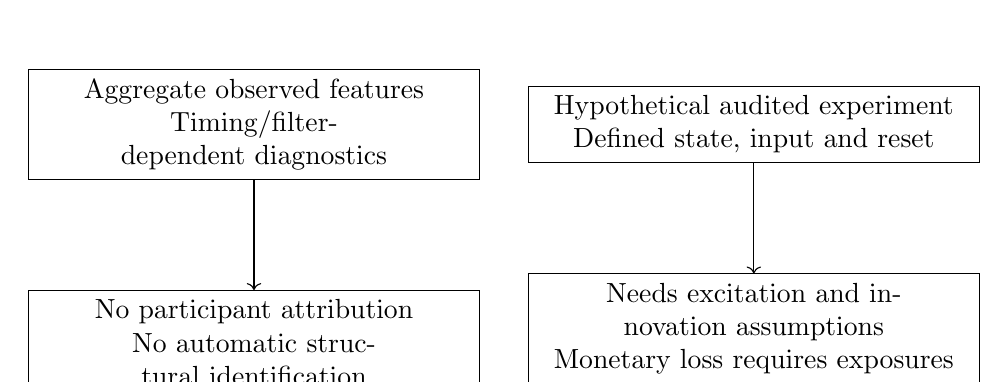
\begin{tikzpicture}[node distance=1.4cm]
\node[draw,align=center,text width=5.5cm] (public) {Aggregate observed features\\Timing/filter-dependent diagnostics};
\node[draw,align=center,text width=5.5cm,right=0.6cm of public] (audit) {Hypothetical audited experiment\\Defined state, input and reset};
\node[draw,align=center,text width=5.5cm,below=of public] (limit) {No participant attribution\\No automatic structural identification};
\node[draw,align=center,text width=5.5cm,below=of audit] (req) {Needs excitation and innovation assumptions\\Monetary loss requires exposures};
\draw[->] (public)--(limit);\draw[->] (audit)--(req);
\end{tikzpicture}
\caption{Information requirements for distinct experiments. Legal audit tags alone do not disclose a learning recursion or authenticate a cash-loss functional.}
\label{fig:surveillance_contracts}\end{figure*}

\subsection{Reconstructed Date-Shuffle, Lead-Flow and Sign Diagnostics}
The previously untraced placebo questions have now been computed under a written retrospective protocol on the existing recorder sample. Date relabelling uses each date's longest continuous segment, position alignment and truncation; all relabellings exclude fixed points. The six-tap price-to-flow regression has a date-mean covariance and is projected onto the negative orthant. That orthant contains the negative Hausdorff-memory cone, so its rejection is a sufficient observable sign restriction diagnostic under the assumed Gaussian covariance law. The diagnostic does not establish that regression taps equal latent algorithm kernels. It does not certify the full continuous-cone test or repair endogenous regressors.
\begin{table}[htbp]
\centering\footnotesize\setlength{\tabcolsep}{3pt}
\caption{Reconstructed recorder diagnostics: 199 fixed-point-free whole-date flow relabellings and 1,999 Gaussian vertex draws for the six-tap negative orthant. The printed ranks are simulation diagnostics at finite resolution, not randomized-treatment or finite-sample market $p$ values.}
\label{tab:falsification}
\resizebox{\textwidth}{!}{\begin{tabular}{lrrr}\toprule
Asset & Date-shuffle rank & Forward-paired $Q$ & Negative-orthant rank \\\midrule
BTC & 0.0050 & 0.0125227 & 0.0005 \\
ETH & 0.0050 & 0.0113018 & 0.0005 \\
ADA & 0.0050 & 0.0072058 & 0.0005 \\
\bottomrule\end{tabular}}
\end{table}

All three shuffle ranks reach the 1/200 simulation floor, and all three Gaussian orthant ranks reach the 1/2000 floor. These are lower-resolution ranks rather than exact zero probabilities. Cross-date exchangeability and the Gaussian covariance reference remain unproved in 13 dates. Lead-flow pairing reproduces the much larger forward diagnostic; it is evidence that timing matters, not a valid exclusion of reverse causation. The independent ledger retains all coefficients, covariances and relabelling indices.

\subsection{Original-Panel Lag Controls and Horizon Units}
The original 768-unit lag grid is newly recomputed from the authenticated current archives. It uses observed flow and complete ten-second bars, without filling or cross-gap regressors. The digital ledger retains every coefficient and denominator as well as date means and intervals. A positive adjusted mean cannot distinguish meta-order execution from adaptive feedback, and finite lag controls do not prove a positive asymptotic floor.
\begin{table}[htbp]
\centering\footnotesize\setlength{\tabcolsep}{3pt}
\caption{Fresh controls on all 768 original study units, using observed flow. $L$ counts ten-second bars: the displayed horizons are 10, 50, 150, 300, 600 and 900 seconds. $L=1$ equals baseline VAR. Date intervals and every segment denominator are retained in the digital ledger.}
\label{tab:lag_memory_controls}
\resizebox{\textwidth}{!}{\begin{tabular}{lrrrrrr}\toprule
Pair & $L=1$ & $L=5$ & $L=15$ & $L=30$ & $L=60$ & $L=90$ \\\midrule
BTC/USDT & 0.0006350 & 0.0006233 & 0.0005719 & 0.0005751 & 0.0006352 & 0.0006545 \\
ETH/USDT & 0.0005657 & 0.0003970 & 0.0003256 & 0.0003358 & 0.0003685 & 0.0003876 \\
SOL/USDT & 0.0002036 & 0.0001401 & 0.0001265 & 0.0001314 & 0.0001270 & 0.0001371 \\
ADA/USDT & 0.0003953 & 0.0003466 & 0.0003536 & 0.0003623 & 0.0003734 & 0.0004001 \\
DOGE/USDT & 0.0002511 & 0.0001911 & 0.0001588 & 0.0001622 & 0.0001604 & 0.0002019 \\
BNB/USDT & 0.0004587 & 0.0003060 & 0.0002888 & 0.0002731 & 0.0003099 & 0.0003253 \\
XRP/USDT & 0.0002292 & 0.0002245 & 0.0001978 & 0.0001741 & 0.0002046 & 0.0002194 \\
LTC/USDT & 0.0003068 & 0.0002120 & 0.0002666 & 0.0002650 & 0.0002881 & 0.0003046 \\
\bottomrule\end{tabular}}
\end{table}

\subsection{Sampling and Filter Sensitivity}
The complete recorder grid reports each computed construction. The mechanical EMA anchor is $1-2/(W/\Delta+1)$ and is distinct from a fitted VAR coefficient. Finite grid comparisons do not establish a universal $O(1/W)$ economic law or robustness to every discretization. Some coarse-clock $Q$ intervals include zero.
\begin{table}[htbp]
\centering\footnotesize\setlength{\tabcolsep}{3pt}
\caption{Complete computed recorder grid: existing BTC/ETH/ADA sample, observed flow, gap-aware filters. Each cell uses 13 dates. Intervals use a retrospective date Student reference; 60-second windows at 60-second sampling are excluded because the filter is degenerate.}
\label{tab:empirical_grid}
\resizebox{\textwidth}{!}{\begin{tabular}{lrrrrrr}\toprule
Asset & $\Delta$ (s) & $W$ (s) & $Q$ & Date interval & $S$ & Date interval \\\midrule
BTC & 1 & 60 & 0.0006658 & [0.0004847, 0.0008469] & 0.9771337 & [0.9762386, 0.9780288] \\
BTC & 1 & 300 & 0.0003072 & [0.0002163, 0.0003982] & 0.9952180 & [0.9949597, 0.9954762] \\
BTC & 1 & 900 & 0.0001660 & [0.0001031, 0.0002288] & 0.9981992 & [0.9981008, 0.9982977] \\
BTC & 10 & 60 & 0.0021823 & [0.0002850, 0.0040796] & 0.7497710 & [0.7362451, 0.7632969] \\
BTC & 10 & 300 & 0.0019353 & [0.0003179, 0.0035527] & 0.9425983 & [0.9388340, 0.9463626] \\
BTC & 10 & 900 & 0.0011979 & [0.0002926, 0.0021032] & 0.9785557 & [0.9768400, 0.9802714] \\
BTC & 60 & 300 & 0.0017936 & [-0.0028178, 0.0064051] & 0.6494995 & [0.6307149, 0.6682842] \\
BTC & 60 & 900 & 0.0017777 & [-0.0024546, 0.0060101] & 0.8562867 & [0.8458932, 0.8666802] \\
ETH & 1 & 60 & 0.0004845 & [0.0002733, 0.0006958] & 0.9728547 & [0.9714421, 0.9742673] \\
ETH & 1 & 300 & 0.0002829 & [0.0001828, 0.0003830] & 0.9941826 & [0.9937325, 0.9946327] \\
ETH & 1 & 900 & 0.0001629 & [0.0000982, 0.0002275] & 0.9978294 & [0.9976065, 0.9980522] \\
ETH & 10 & 60 & 0.0011250 & [-0.0001413, 0.0023913] & 0.7299855 & [0.7150779, 0.7448931] \\
ETH & 10 & 300 & 0.0009795 & [0.0000628, 0.0018963] & 0.9391562 & [0.9338698, 0.9444427] \\
ETH & 10 & 900 & 0.0007203 & [0.0000851, 0.0013554] & 0.9781093 & [0.9759674, 0.9802512] \\
ETH & 60 & 300 & -0.0027069 & [-0.0078037, 0.0023900] & 0.6705125 & [0.6512727, 0.6897523] \\
ETH & 60 & 900 & -0.0009565 & [-0.0048536, 0.0029407] & 0.8679761 & [0.8593363, 0.8766159] \\
ADA & 1 & 60 & 0.0002474 & [0.0001359, 0.0003589] & 0.9705855 & [0.9686803, 0.9724907] \\
ADA & 1 & 300 & 0.0001361 & [0.0000809, 0.0001913] & 0.9935311 & [0.9930170, 0.9940453] \\
ADA & 1 & 900 & 0.0000793 & [0.0000438, 0.0001148] & 0.9974690 & [0.9971371, 0.9978008] \\
ADA & 10 & 60 & 0.0007698 & [0.0001114, 0.0014281] & 0.7232232 & [0.7138175, 0.7326289] \\
ADA & 10 & 300 & 0.0006163 & [0.0001565, 0.0010762] & 0.9350377 & [0.9304137, 0.9396617] \\
ADA & 10 & 900 & 0.0003875 & [0.0000696, 0.0007053] & 0.9763042 & [0.9741121, 0.9784963] \\
ADA & 60 & 300 & 0.0016322 & [-0.0006946, 0.0039589] & 0.6486999 & [0.6276182, 0.6697817] \\
ADA & 60 & 900 & 0.0014004 & [-0.0007271, 0.0035280] & 0.8586178 & [0.8480483, 0.8691874] \\
\bottomrule\end{tabular}}
\end{table}

\subsection{January Depth and Retrospective Forecasts}
The January sample has 3,730,870 raw snapshots spanning January 9--20, 2023. Top-quote OFI and the 120-second EMA yield 844,621 valid transitions in 152 segments over 12 dates. The mean is $Q=0.000910232$. The controlled diagnostic is $Q_{30}=-0.001296032$, with date interval $[-0.001567464,-0.001024600]$. The CSV exactly matches a Parquet-to-CSV reconstruction of the named primary distribution. Its uploader declares Apache 2.0, while exchange/contract details remain undocumented. The sample was previously examined; it is not an untouched prospective holdout. A fresh retrospective AR/VAR comparison now reconstructs this same sample, matching all 152 prior eligible segments and 844,621 baseline transitions. Training-only normalization and fitting precede six expanding evaluation dates, January 15--20, 2023. At lags one, two, three and six seconds, mean price-MSE reductions are 1.84275, 1.78394, 1.77683 and 1.75939 percent relative to AR. All four date-Student reference intervals are positive. With only six consecutive evaluation dates, retrospective choices and serial dependence, these are predictive associations rather than guaranteed confidence coverage or causal learning identification. Every lag and both price/flow loss targets are retained. Non-rejection neither proves equal prediction nor validates a learning mechanism.


\section{Regulatory Policy Implications and Conclusion}
\label{sec:policy_conclusion}

\subsection{Pre-Trade Controls and the Scope of the Proposed Bound}
Existing market-access rules already include pre-trade controls. SEC Rule 15c3-5 requires controls against orders exceeding appropriate credit/capital thresholds and erroneous orders; the SEC staff FAQ discusses their application to quotes and automated activity \citep{sec2010marketaccess,sec2017marketaccessfaq}. The present mathematical bound is a conditional design input. Its derivation does not establish regulatory compliance, improved welfare or an implemented exchange safety mechanism.

\subsection{An Explicit Finite-Window Quantity Gate}
An initial-state norm radius alone does not specify an executed-volume limit. Let $v_j$ be signed executed quantity, $H$ its input map and $Cz$ a financially specified monetary loss output:
\[
z_{j+1}=Jz_j+Hv_j,\qquad \ell_t=Cz_t,
\qquad \sum_{j=0}^{N-1}|v_j|\le V.
\]
Set $b_t=CJ^tz_0$ and $g_t=\max_{0\le k<t}|CJ^kH|$. Under an absolute-output budget, the sharp finite-window envelope is $|b_t|+L_{\rm other}+(g_t+c_{\rm exec})V$, where $L_{\rm other}$ is a declared monetary reserve and $c_{\rm exec}$ bounds monetary cost per executed quantity. Provided all background outputs, including $t=0$, are within budget, the cap is
\begin{equation}
\bar R=\frac{V^*}{\tau},\qquad
V^*=\min_{\substack{1\le t\le N\\g_t+c_{\rm exec}>0}}
\frac{B-L_{\rm other}-|b_t|}{g_t+c_{\rm exec}},
\label{eq:rate_gating_rule}
\end{equation}
for a window lasting $\tau$ seconds. This is quantity per second, not order-message count. Zero-gain times impose no quantity restriction if their background is feasible; an already exceeded background cannot be certified by setting a cap to zero. No Schur condition is needed for this finite-horizon calculation.

\begin{proof}
Superposition yields $\ell_t=b_t+\sum_{j<t}CJ^{t-1-j}Hv_j$. The maximum coefficient bounds the input term by $g_tV$; an adversarial single pulse at its maximizing lag attains the bound under the declared quantity ball. Costs add at most $c_{\rm exec}V$. Taking the minimum over every time gives the largest permitted cap for this linear criterion. The signed one-sided loss variant replaces $|b_t|$ with $b_t$.
\end{proof}

The Markov coefficients and this cap are unchanged by consistent invertible changes of state coordinates. The old map $\|z_0\|\le|x_0|$ is unsupported for a state with unobserved cohort components; the price component alone is a lower, not upper, bound on its Euclidean norm. Displayed top-five quantity and price impact do not determine $H$, and leveraged notional is not loss-absorbing capital.

Cohort nonidentification does not by itself make every financial functional unknown. For two reset models with identical price input responses and the same calibrated monetary price exposure, equality of Markov coefficients gives identical finite-window caps even when cohort counts differ. This is an input/output functional, not a first-use control result. Unreset hidden states, unknown exposure/input maps, nonlinear marks and changing positions require additional information.

In the one-asset positive-cohort model with $S=a+\kappa\sum_iq_i<1$, a reset price-only monetary output has executed-input peak $|\lambda|\kappa$, while its sustained-input gain is $|\lambda|\kappa/(1-S)$. Nonnegative row sums and the DC response prove this distinction. It requires the stated fixed output, input and model conditions; it does not include fundamental risk or accumulated costs. The all-state initial-shock norm and the physical execution-input risk can rank impact changes differently. The supplement gives an exact example in which the state norm falls while execution gain rises. These disturbance/output contracts must therefore be specified before interpreting a non-normality metric financially.

Each refreshed window must carry the actual state and updated capital, cost and uncertainty bounds. With $z_{t+1}=0.9z_t+v_t$ and budget one, two unit pulses in consecutive one-step windows produce output 1.9; carrying the first state reduces the second permitted pulse to 0.1. Thus window resets do not establish perpetual solvency. The detailed proof, coordinate/unit checks and exact failure examples are in the input-gate supplement. Operational use still requires authenticated positions, marks, executions, fees/funding/margin rules and model/noise/input coverage. The empirical maintained-model rejections are not cured by this conditional formula.

\subsection{Market Design: Continuous Auctions vs.\ Frequent Batch Auctions}
Our findings also speak directly to the structural debate on market design initiated by \citet{budish2015}, who propose replacing continuous double auctions with Frequent Batch Auctions (FBAs) to eliminate latency arbitrage. Batch matching changes execution timing and incentives; a feedback model can also be posed across successive batches. This paper does not estimate its comparative economic effect. The finite-window quantity bound can be examined under either matching design when its input/output and accounting assumptions hold. Comparative welfare, execution feasibility and effectiveness across continuous and batch auctions remain unvalidated.

\subsection{Information Missing from Public Market Feeds}
\label{sec:missing_info}
Each result uses a declared information contract. Exact reset response functions determine a merged representation rather than participant identities. Noisy-price testing costs require the stated innovation law and exclusion of richer financial records. Exact marked equity and natural excitation supply constructive counterexamples to a universal capital barrier. The positive-class quantity certificate requires authenticated impact, margin and account assumptions; it does not require individual learning-rate identities once that model class is verified. Covariance rejection and measurement sensitivity prevent substituting public reduced-form coefficients for these operational conditions.

\subsection{Conclusion}
We establish a resource distinction within a precisely defined memory-resolution experiment: lifetime executed quantity of order $\delta^{-2}$ is necessary and sufficient for a known symmetric pair, while average power gives horizon order $\delta^{-4}$. Actual probe-trader execution cost gives matching capital order $\delta^{-4}$ for funded deterministic probes under the restricted noisy-price contract. A separate counterparty cash/margin contract gives a sharp quantity allowance, including the inventory created by the probe. Exact equity disclosure and natural excitation supply constructive counterexamples to a universal capital barrier. A fixed price-exposure output is a separate contract. More waiting alone cannot overcome a fixed lifetime quantity allowance; the result does not bound every tailored safe strategy. The empirical reconstruction shows strong timing/filter sensitivity and maintained-model rejection, rather than participant-level learning attribution. Existing simulations distinguish capacity events, defaults and effective dynamics. Real-market financial calibration and independent specialist assessment remain necessary before publication and operational claims.

\newpage
\begin{thebibliography}{99}
\small
\setlength{\itemsep}{0.0pt plus 0.3pt}
\setlength{\parsep}{0.0pt}

\bibitem[Adrian and Shin(2010)]{adrian2010liquidity}
Adrian, T., and H.~S. Shin, 2010, Liquidity and leverage, \emph{Journal of Financial Intermediation} 19, 418--437.

\bibitem[Almgren and Chriss(2001)]{almgren2000}
Almgren, R., and N.~Chriss, 2001, Optimal execution of portfolio transactions, \emph{Journal of Risk} 3, 5--39.

\bibitem[Andrews(1991)]{andrews1991heteroskedasticity}
Andrews, D.~W., 1991, Heteroskedasticity and autocorrelation consistent covariance matrix estimation, \emph{Econometrica} 59, 817--858.

\bibitem[Avellaneda and Stoikov(2008)]{avellaneda2008high}
Avellaneda, M., and S.~Stoikov, 2008, High-frequency trading in a limit order book, \emph{Quantitative Finance} 8, 217--224.

\bibitem[Biais, Foucault, and Moinas(2015)]{biais2015}
Biais, B., T.~Foucault, and S.~Moinas, 2015, Equilibrium fast trading, \emph{Journal of Financial Economics} 116, 292--313.

\bibitem[Bouchaud et~al.(2004)]{bouchaud2004fluctuations}
Bouchaud, J.-P., Y.~Gefen, M.~Potters, and M.~Wyart, 2004, Fluctuations and response in financial markets: The subtle nature of ``random'' price changes, \emph{Quantitative Finance} 4, 176--185.

\bibitem[Brunnermeier and Pedersen(2009)]{brunnermeier2009}
Brunnermeier, M.~K., and L.~H. Pedersen, 2009, Market liquidity and funding liquidity, \emph{Review of Financial Studies} 22, 2201--2238.

\bibitem[Budish, Cramton, and Shim(2015)]{budish2015}
Budish, E., P.~Cramton, and J.~Shim, 2015, The high-frequency trading arms race: Frequent batch auctions as a market design response, \emph{Quarterly Journal of Economics} 130, 1547--1621.

\bibitem[Campbell, Grossman, and Wang(1993)]{campbell1993trading}
Campbell, J.~Y., S.~J. Grossman, and J.~Wang, 1993, Trading volume and serial correlation in stock returns, \emph{Quarterly Journal of Economics} 108, 905--939.

\bibitem[CFTC-SEC(2010)]{cftc_sec_2010}
CFTC and SEC, 2010, Findings regarding the market events of May 6, 2010: Report of the staffs of the CFTC and SEC to the Joint Advisory Committee on Emerging Regulatory Issues, Technical report, Commodity Futures Trading Commission and Securities and Exchange Commission.

\bibitem[Cont, Stoikov, and Talreja(2010)]{cont2010stochastic}
Cont, R., S.~Stoikov, and R.~Talreja, 2010, A stochastic model for order book dynamics, \emph{Operations Research} 58, 549--563.

\bibitem[Cont, Kukanov, and Stoikov(2014)]{cont2014}
Cont, R., A.~Kukanov, and S.~Stoikov, 2014, The price impact of order book events, \emph{Journal of Financial Econometrics} 12, 47--88.

\bibitem[Donald and Lang(2007)]{donald2007inference}
Donald, S.~G., and K.~Lang, 2007, Inference with difference-in-differences and other panel data, \emph{Review of Economics and Statistics} 89, 221--233.

\bibitem[Eisenberg and Noe(2001)]{eisenberg2001systemic}
Eisenberg, L., and T.~H. Noe, 2001, Systemic risk in financial systems, \emph{Management Science} 47, 236--249.

\bibitem[Epstein and Schneider(2008)]{epstein2008ambiguity}
Epstein, L.~G., and M.~Schneider, 2008, Ambiguity, information quality, and asset pricing, \emph{Journal of Finance} 63, 197--228.

\bibitem[Gilbert(1963)]{gilbert1963}
Gilbert, E.~G., 1963, Controllability and observability in multivariable control systems, \emph{Journal of the Society for Industrial and Applied Mathematics, Series A: Control} 1, 128--151.

\bibitem[Gilboa and Schmeidler(1989)]{gilboa1989maxmin}
Gilboa, I., and D.~Schmeidler, 1989, Maxmin expected utility with non-unique prior, \emph{Journal of Mathematical Economics} 18, 141--153.

\bibitem[Glosten and Milgrom(1985)]{glosten1985bid}
Glosten, L.~R., and P.~R. Milgrom, 1985, Bid, ask and transaction prices in a specialist market with heterogeneously informed traders, \emph{Journal of Financial Economics} 14, 71--100.

\bibitem[Greenwood, Landier, and Thesmar(2015)]{greenwood2015vulnerable}
Greenwood, R., A.~Landier, and D.~Thesmar, 2015, Vulnerable banks, \emph{Journal of Financial Economics} 115, 471--485.

\bibitem[Grossman and Miller(1988)]{grossman1988liquidity}
Grossman, S.~J., and M.~H. Miller, 1988, Liquidity and market structure, \emph{Journal of Finance} 43, 617--633.

\bibitem[Hasbrouck(1991)]{hasbrouck1991}
Hasbrouck, J., 1991, Measuring the information content of stock trades, \emph{Journal of Finance} 46, 179--207.

\bibitem[He and Krishnamurthy(2013)]{he2013intermediary}
He, Z., and A.~Krishnamurthy, 2013, Intermediary asset pricing, \emph{American Economic Review} 103, 732--773.

\bibitem[Hendershott, Jones, and Menkveld(2011)]{hendershott2011does}
Hendershott, T., C.~M. Jones, and A.~J. Menkveld, 2011, Does algorithmic trading improve liquidity?, \emph{Journal of Finance} 66, 1--33.

\bibitem[Ho and Stoll(1981)]{ho1981optimal}
Ho, T., and H.~R. Stoll, 1981, Optimal dealer pricing under transactions and return uncertainty, \emph{Journal of Financial Economics} 9, 47--73.

\bibitem[Joint Treasury Staff(2015)]{joint_treasury_2015}
Joint Treasury Staff, 2015, The U.S. Treasury market on October 15, 2014, Staff report, U.S. Department of the Treasury, Board of Governors of the Federal Reserve System, Federal Reserve Bank of New York, Securities and Exchange Commission, and Commodity Futures Trading Commission.

\bibitem[Kalman(1960)]{kalman1960}
Kalman, R.~E., 1960, A new approach to linear filtering and prediction problems, \emph{Journal of Basic Engineering} 82, 35--45.

\bibitem[Kreiss(1962)]{kreiss1962}
Kreiss, H.-O., 1962, {\"U}ber die Stabilit{\"a}tsdefinition f{\"u}r Differenzengleichungen die partielle Differentialgleichungen approximieren, \emph{BIT Numerical Mathematics} 2, 153--181.

\bibitem[Kyle(1985)]{kyle1985continuous}
Kyle, A.~S., 1985, Continuous auctions and informed trader, \emph{Econometrica} 53, 1315--1335.

\bibitem[Le Cam(1986)]{lecam1986}
Le Cam, L., 1986, \emph{Asymptotic Methods in Statistical Decision Theory}, Springer-Verlag.

\bibitem[MacKinnon and Webb(2018)]{mackinnon2018wild}
MacKinnon, J.~G., and M.~D. Webb, 2018, The wild bootstrap for few (treated) clusters, \emph{Econometrics Journal} 21, 114--135.

\bibitem[Menkveld(2013)]{menkveld2013}
Menkveld, A.~J., 2013, High frequency trading and the new market makers, \emph{Journal of Financial Markets} 16, 712--740.

\bibitem[Newey and West(1987)]{newey1987simple}
Newey, W.~K., and K.~D. West, 1987, A simple, positive semi-definite, heteroskedasticity and autocorrelation consistent covariance matrix, \emph{Econometrica} 55, 703--708.

\bibitem[Nielsen(2021)]{crypto_rl_2021}
Nielsen, M. S., 2021, High Frequency Crypto Limit Order Book Data, Kaggle dataset version 1, uploader-declared CC0, \url{https://www.kaggle.com/datasets/martinsn/high-frequency-crypto-limit-order-book-data}.

\bibitem[Ntakaris et~al.(2018)]{ntakaris2018benchmark}
Ntakaris, A., M.~Magris, J.~Kanniainen, M.~Gabbouj, and A.~Iosifidis, 2018, Benchmark dataset for mid-price forecasting of limit order book data with machine learning methods, \emph{Journal of Forecasting} 37, 852--866, doi:10.1002/for.2543.

\bibitem[Pesaran and Shin(1998)]{pesaran1998}
Pesaran, H.~H., and Y.~Shin, 1998, Generalized impulse response analysis in linear multivariate models, \emph{Economics Letters} 58, 17--29.

\bibitem[Phillips(1987)]{phillips1987time}
Phillips, P.~C.~B., 1987, Time series regression with a unit root, \emph{Econometrica} 55, 277--301.

\bibitem[Rigobon(2003)]{rigobon2003identification}
Rigobon, R., 2003, Identification through heteroskedasticity, \emph{Review of Economics and Statistics} 85, 777--792.

\bibitem[Spijker(1991)]{spijker1991}
Spijker, M.~N., 1991, On a conjecture by LeVeque and Trefethen related to the Kreiss matrix theorem, \emph{BIT Numerical Mathematics} 31, 551--555.

\bibitem[Trefethen and Embree(2005)]{trefethen2005spectra}
Trefethen, L.~N., and M.~Embree, 2005, \emph{Spectra and Pseudospectra: The Behavior of Nonnormal Matrices and Operators}, Princeton University Press.


\bibitem[SEC(2010)]{sec2010marketaccess}
U.S. Securities and Exchange Commission, 2010, Risk Management Controls for Brokers or Dealers with Market Access, Release No.34-63241, \url{https://www.sec.gov/rules/final/2010/34-63241.pdf}.
\bibitem[SEC Staff(2017)]{sec2017marketaccessfaq}
SEC Division of Trading and Markets, 2017, Responses to Frequently Asked Questions Concerning Risk Management Controls for Brokers or Dealers with Market Access, staff guidance, \url{https://www.sec.gov/rules-regulations/staff-guidance/trading-markets-frequently-asked-questions/divisionsmarketregfaq-0}.


\bibitem[Liu and Ammari(2023)]{liuammari2023}
Liu, P., and H. Ammari, 2023, Super-resolution of positive near-colliding point sources, \emph{Information and Inference} 12, primary preprint arXiv:2212.00536.
\bibitem[Manole and Ho(2022)]{manoleho2022}
Manole, T., and N. Ho, 2022, Refined convergence rates for maximum likelihood estimation under finite mixture models, \emph{Proceedings of Machine Learning Research} 162, 14979--15006.
\bibitem[Sornette et al.(2023)]{sornette2023nonnormal}
Sornette, D., S. Lera, J. Lin, and K. Wu, 2023, Non-normal interactions create socio-economic bubbles, primary manuscript arXiv:2205.08661v5.

\bibitem[Park and Van Roy(2012)]{parkvanroy2012}
Park, B., and B. Van Roy, 2012, Adaptive execution: Exploration and learning of price impact, primary preprint arXiv:1207.6423.
\bibitem[Gatheral(2010)]{gatheral2010}
Gatheral, J., 2010, No-dynamic-arbitrage and market impact, \emph{Quantitative Finance} 10, 749--759, doi:10.1080/14697680903373692.
\bibitem[Schneider and Lillo(2017)]{schneiderlillo2017}
Schneider, M., and F. Lillo, 2017, Cross-impact and no-dynamic-arbitrage, primary preprint arXiv:1612.07742v2.

\bibitem[Li et al.(2024)]{li2024trajectory}
Li, F., V. Ihnatiuk, Y. Chen, J. Lin, R. J. Kinnear, A. Schneider, Y. Nevmyvaka, and H. Lam, 2024, Do price trajectory data increase the efficiency of market impact estimation?, \emph{Quantitative Finance} 24, 545--568, doi:10.1080/14697688.2024.2351457.
\bibitem[Alfonsi et al.(2016)]{alfonsi2016matrix}
Alfonsi, A., A. Schied, and F. Kl\"ock, 2016, Multivariate transient price impact and matrix-valued positive definite functions, \emph{Mathematics of Operations Research} 41, 914--934; primary preprint arXiv:1310.4471.

\bibitem[Chatzikiriakos and Iannelli(2024)]{chatzikiriakos2024finite}
Chatzikiriakos, N., and A. Iannelli, 2024, Sample complexity bounds for linear system identification from a finite set, \emph{IEEE Control Systems Letters}; primary author manuscript.
\bibitem[Chatzikiriakos et al.(2026)]{chatzikiriakos2026active}
Chatzikiriakos, N., K. Jamieson, and A. Iannelli, 2026, High effort, low gain: Fundamental limits of active learning for linear dynamical systems, \emph{Proceedings of Machine Learning Research} 300, 3115--3123.

\end{thebibliography}

\end{document}
